\documentclass[11pt,dvipdfmx]{jarticle}
\usepackage{eee}


\begin{document}
\begin{jikkenTitle}
\gakunen{3} 
\numTitle{0}{RLC回路におけるインピーダンス軌跡の特定} 
\subTitle{(Elucidating the impedance locus under the RLC circuit)} 
\jikkenbi{令和04年4月14日(木)} 
\yoteibi{04/28}
\yoteibiII{05/12}
\hanNumberName{09}{3309}{大山 主朗} 
\end{jikkenTitle}


\section{目的}
計測器では計測することのできない電気回路の複素数の性質を,回路を計測した値を用いて計算することにより,極座標に表示させる.
\section{原理}
直列回路では電流が一定.並列回路では電圧が一定.
\section{方法}
\subsection{実験装置}
\space 実験には以下のものを使用する.
\begin{table}[hbtp]
  \centering
  \caption{実験装置}
  \label{tab:1}
  \begin{tabular}{cc}
    \hline
    機器名&数量[個]\\
    \hline
    ファンクション・ジェネレータ&1\\
    1000[$\Omega$]の抵抗&1\\
    2[$mH$]のインダクタ&1\\
    5[$mH$]のインダクタ&1\\
    2.25[$\mu F$]のキャパシタ&1\\
    250[$\mu F$]のキャパシタ&1\\
    交流用電流計&3\\
    交流用電圧計&3\\
    \hline
  \end{tabular}
\end{table}
\subsection{実験手順(直列回路)}
\begin{enumerate}
\begin{figure}[hptb]
 \centering
 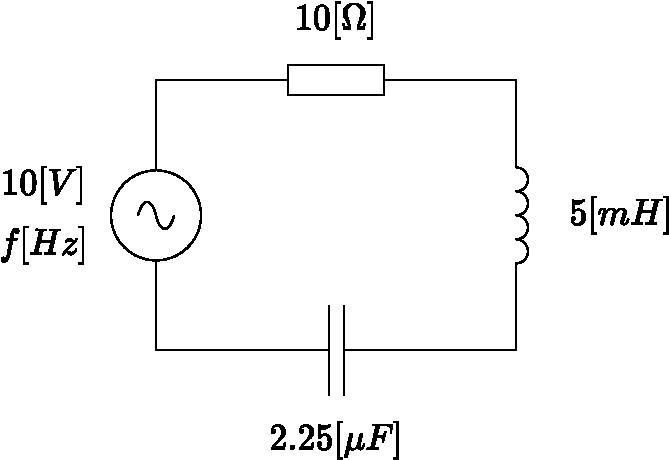
\includegraphics[scale=0.7]{./fig/fig1.pdf}
 \caption{RLC直列回路}
 \label{fig:1}
\end{figure}
\item \wpfig{1}のように回路を構築する.
\begin{figure}
 \centering
 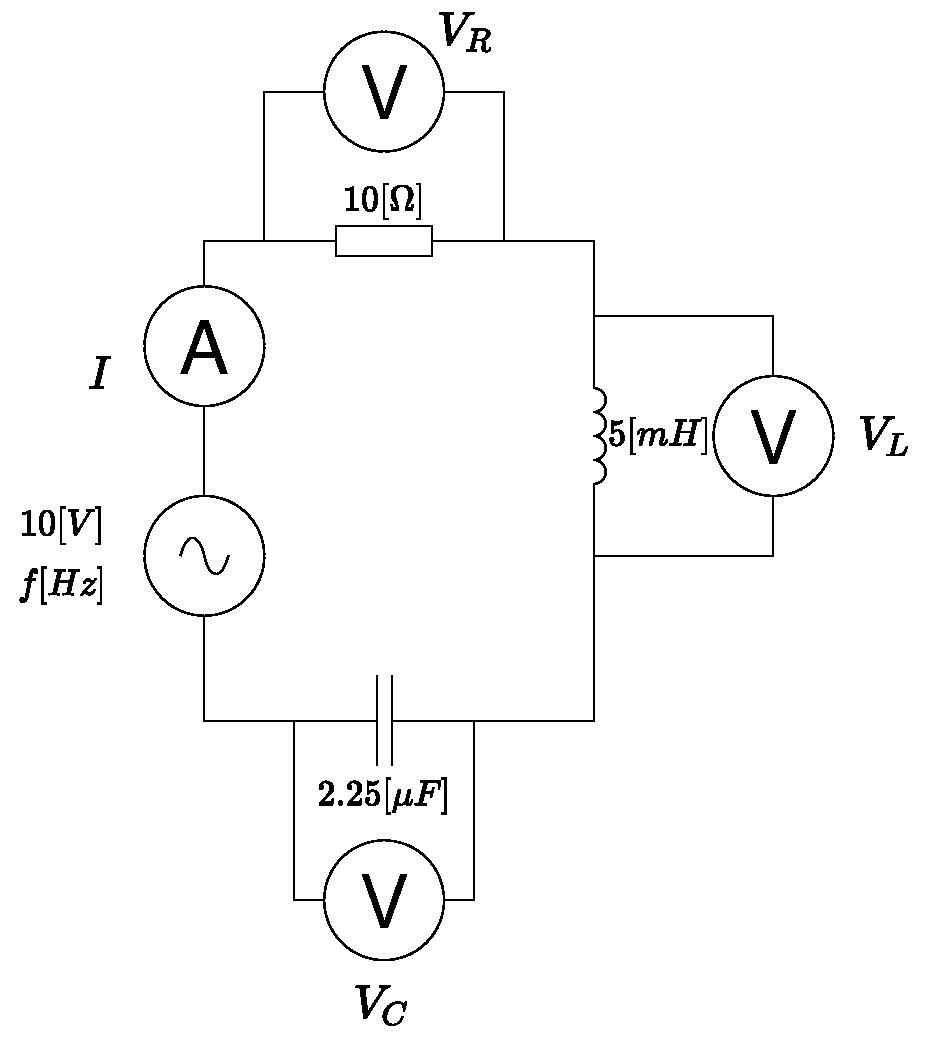
\includegraphics[scale=0.5]{./fig/fig3.pdf}
 \caption{RLC直列回路}
 \label{fig:fig3}
\end{figure}
\item \wpfig{fig3}を参考に交流用電流計および,交流用電圧計を設置する.
\item 周波数を$500[Hz]$から$5000[Hz]$まで$400[Hz]$おきに変化させ,$V_R,V_L,V_C$及び$I$の値を記録する.
\item 上で測定した値を要素が周波数・インピーダンスの大きさ・偏角である表にまとめる.\\
なお,インピーダンスの大きさは\wpeq{1},偏角は\wpeq{2}で算出することができる.
\begin{align}
\label{eq:1}
|Z_s|&=\frac{V_R+V_L+V_C}{I}[\Omega]\\
\label{eq:2}
\theta_s&=\tan^{-1}\left(\frac{V_L-V_C}{V_R}\right)[rad]
\end{align}
\item 計算したインピーダンスの大きさ・偏角および,\wpeq{8}を用いてインピーダンスの軌跡を描画する.
\begin{equation}
\label{eq:8}
実部=|Z|\cos \theta_p \qquad 虚部=|Z|\sin \theta_p 
\end{equation}
\end{enumerate}
\subsection{実験手順(並列回路)}
\begin{enumerate}
\begin{figure}
 \centering
 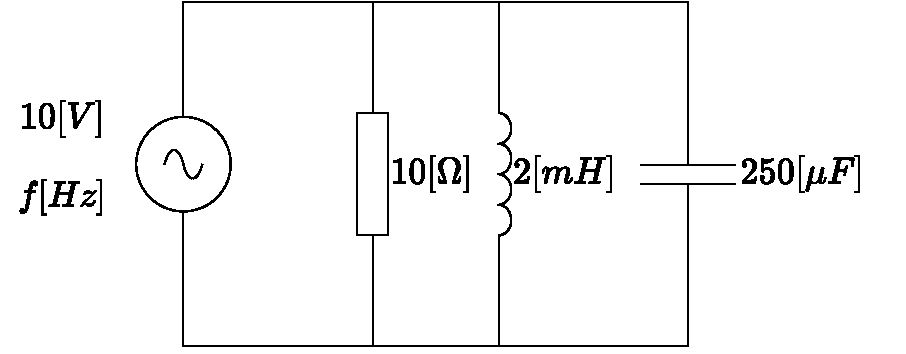
\includegraphics[scale=0.7]{./fig/fig2.pdf}
 \caption{RLC並列回路}
 \label{fig:fig2}
\end{figure}
\item \wpfig{fig2}のように回路を構築する.
\begin{figure}
 \centering
 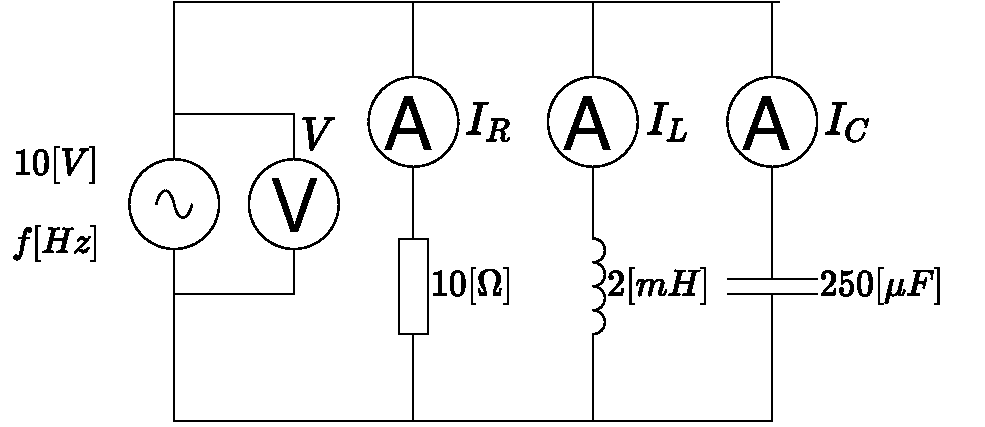
\includegraphics[scale=0.5]{./fig/fig4.pdf}
 \caption{RLC直列回路}
 \label{fig:fig4}
\end{figure}
\item \wpfig{fig4}を参考に交流用電流計および,交流用電圧計を設置する.
\item 周波数を$500[Hz]$から$5000[Hz]$まで$10[Hz]$おきに変化させ,$I_R,I_L,I_C$及び$V$の値を記録する.
\item 上で測定した値を要素が周波数・インピーダンスの大きさ・偏角である表にまとめる.\\
なお,インピーダンスの大きさは式\wpeq{3},偏角は式\wpeq{4}で算出することができる.
\begin{align}
\label{eq:3}
|Z_p|&=\frac{V}{I_R+I_L+I_C}[\Omega]\\
\label{eq:4}
\theta_p&=\tan^{-1}\left(\frac{I_L-I_C}{I_{R}}\right)[rad]
\end{align}
\item 計算したインピーダンスの大きさ・偏角および,\wpeq{8}を用いてインピーダンスの軌跡を描画する.
\end{enumerate}
\section{結果}
\subsection{直列回路}
\begin{enumerate}
\item 測定値により導出された特性値の変化を\wptab{2}に示す.なお,インピーダンス及び偏角の値はexcelを用いて算出した.
また計算値は,小数第4位で四捨五入した.\\
$1700[Hz]$がインピーダンス,偏角ともに最小値であり,$1700[Hz]$近傍の変化率が高周波付近より大きいことがわかる.
\begin{table}[hbtp]
  \centering
  \caption{インピーダンス・偏角の周波数特性(直列)}
  \label{tab:2}
  \begin{tabular}{ccc}
    \hline
    周波数$[Hz]$&インピーダンス[$\Omega$]&偏角[$rad$]\\
    \hline
    500  & 126.061 & -1.491 \\
    900  & 51.251 & -1.374 \\
    1300 & 16.827 & -0.935 \\
    1700 & 15.488 & 0.869 \\
    2100 & 33.825 & 1.271 \\
    2500 & 51.251 & 1.374 \\
    2900 & 67.477 & 1.422 \\
    3300 & 82.858 & 1.450 \\
    3700 & 97.648 & 1.468 \\
    4100 & 112.012 & 1.481 \\
    4500 & 126.061 & 1.491 \\
    4900 & 139.870 & 1.499 \\
    5300 & 153.494 & 1.506 \\
    5700 & 166.970 & 1.511 \\
    6100 & 180.327 & 1.515 \\
    6500 & 193.587 & 1.519 \\
    \hline
  \end{tabular}
\end{table}
\item RLC回路の共振周波数は\wpeq{5}より$1500[Hz]$であり,\wptab{2}でインピーダンス・偏角の値が,$1500[Hz]$近傍で抵抗の特性(偏角が0・インピーダンスが抵抗値)に近づいていることがわかる.\\
よって理論との一致が確認できた.
\begin{align}
\label{eq:5}
f_0&=\frac{1}{2\pi \sqrt{LC}}=\frac{1}{2\pi \sqrt{5\times 10^{-3}\cdot 2.25\times 10^{-6}}} \fallingdotseq 1500[Hz]
\end{align}
\item \wptab{2}の周波数によるインピーダンスの変化を,近似曲線と重ねて\wpfig{fig5}に示す.\\
共振周波数より大きい周波数では滑らかにインピーダンスの値が増加している.
\begin{figure}
 \centering
 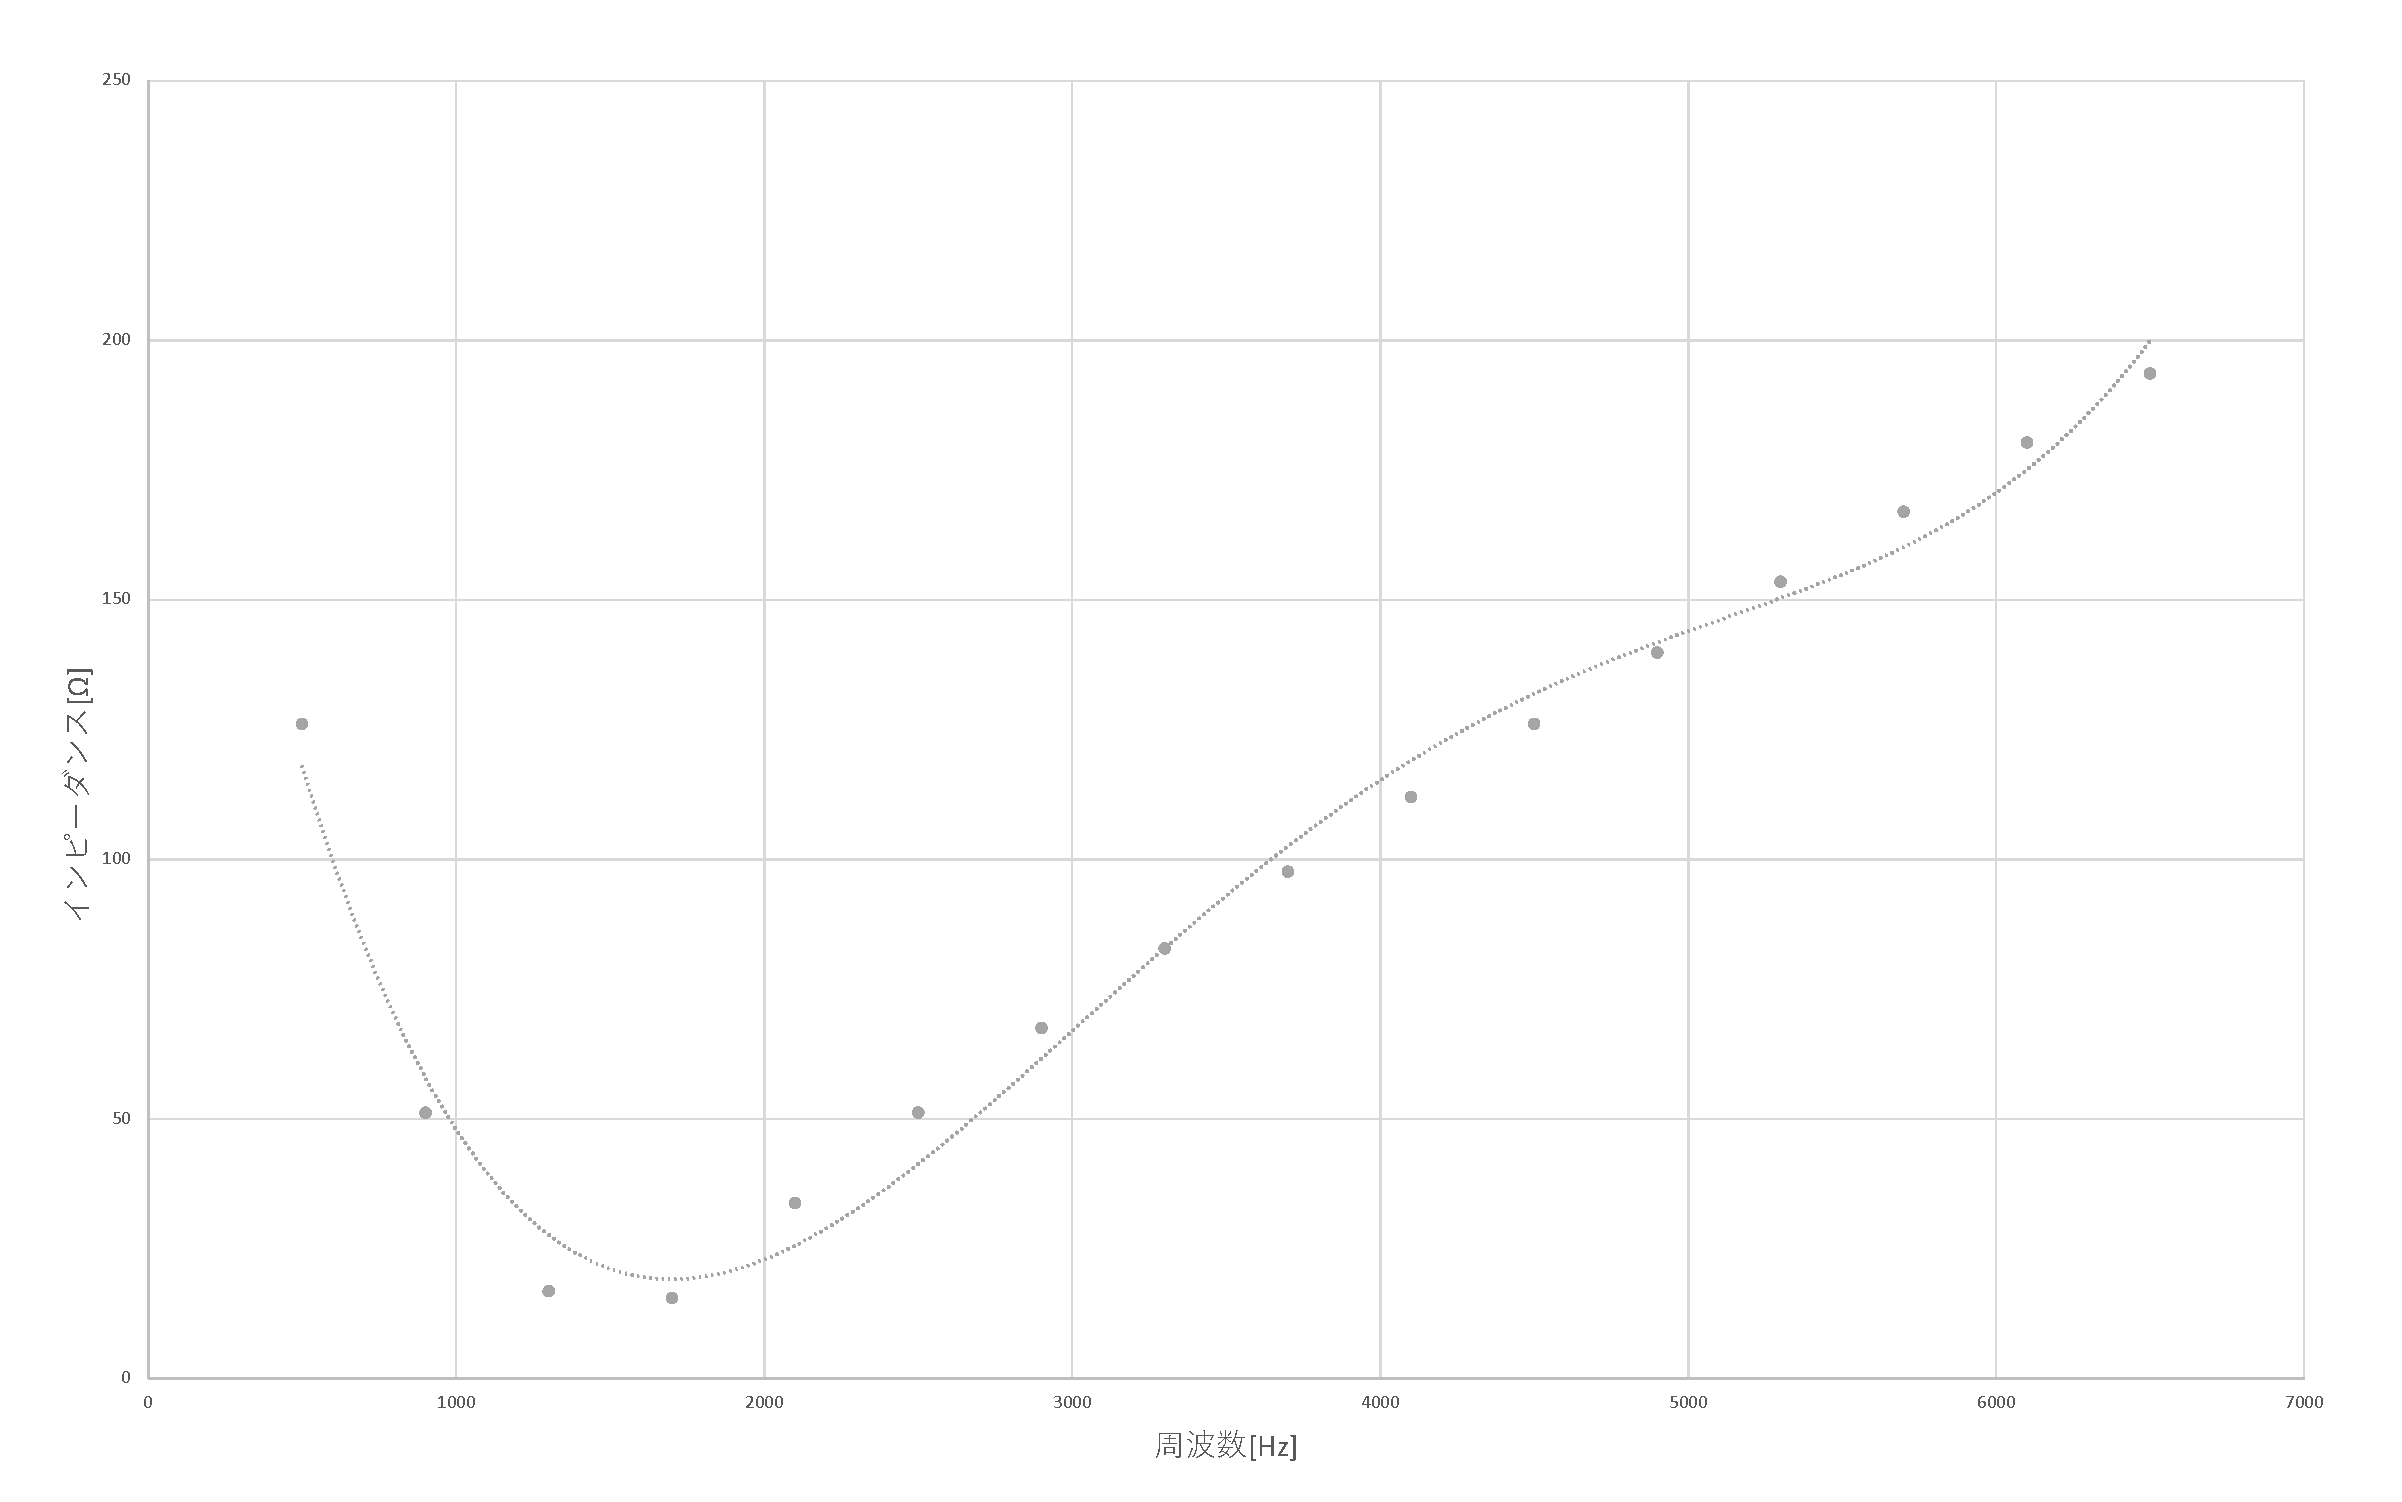
\includegraphics[scale=0.45]{./fig/graph1.pdf}
 \caption{インピーダンスの大きさの周波数特性(直列)}
 \label{fig:fig5}
\end{figure}
\item \wpfig{fig6}は偏角の周波数特性を近似直線とともに,グラフにしたものである.\\
高周波では偏角の変化が少なく,共振周波数付近で大きく変化していることがわかる.
\begin{figure}
 \centering
 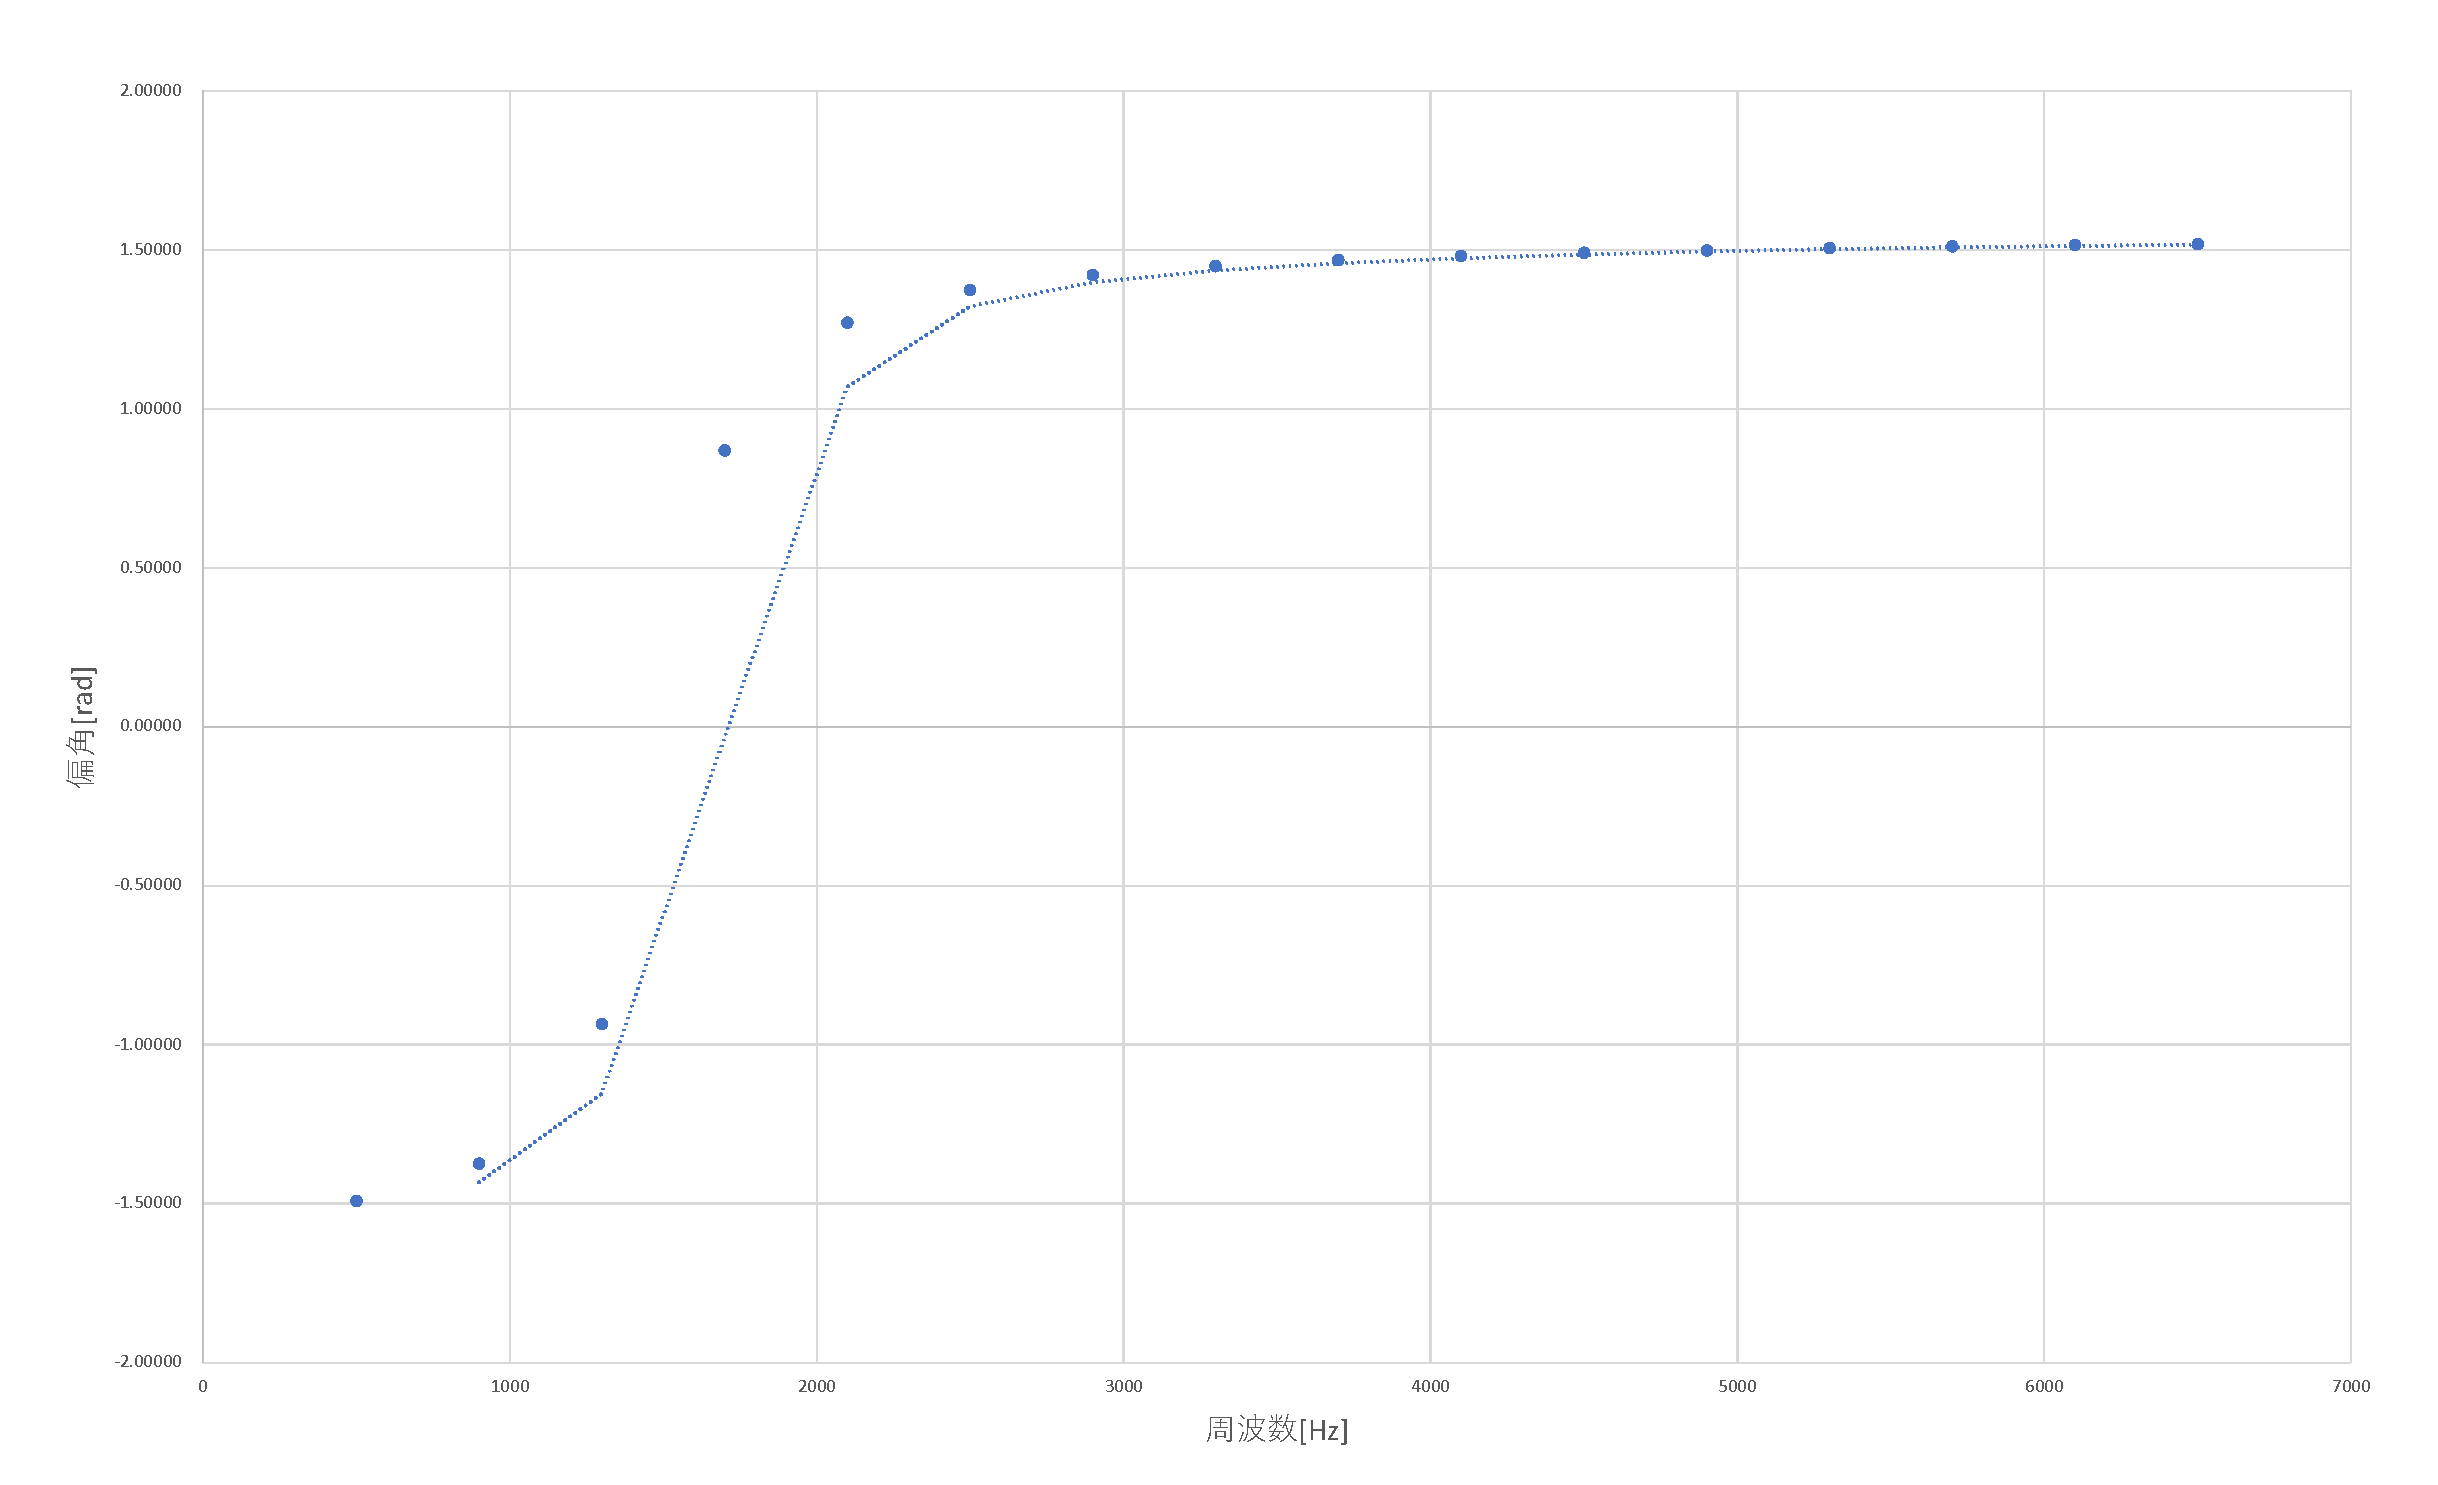
\includegraphics[scale=0.45]{./fig/graph2.pdf}
 \caption{偏角の周波数特性(直列)}
 \label{fig:fig6}
\end{figure}
\begin{figure}
 \centering
 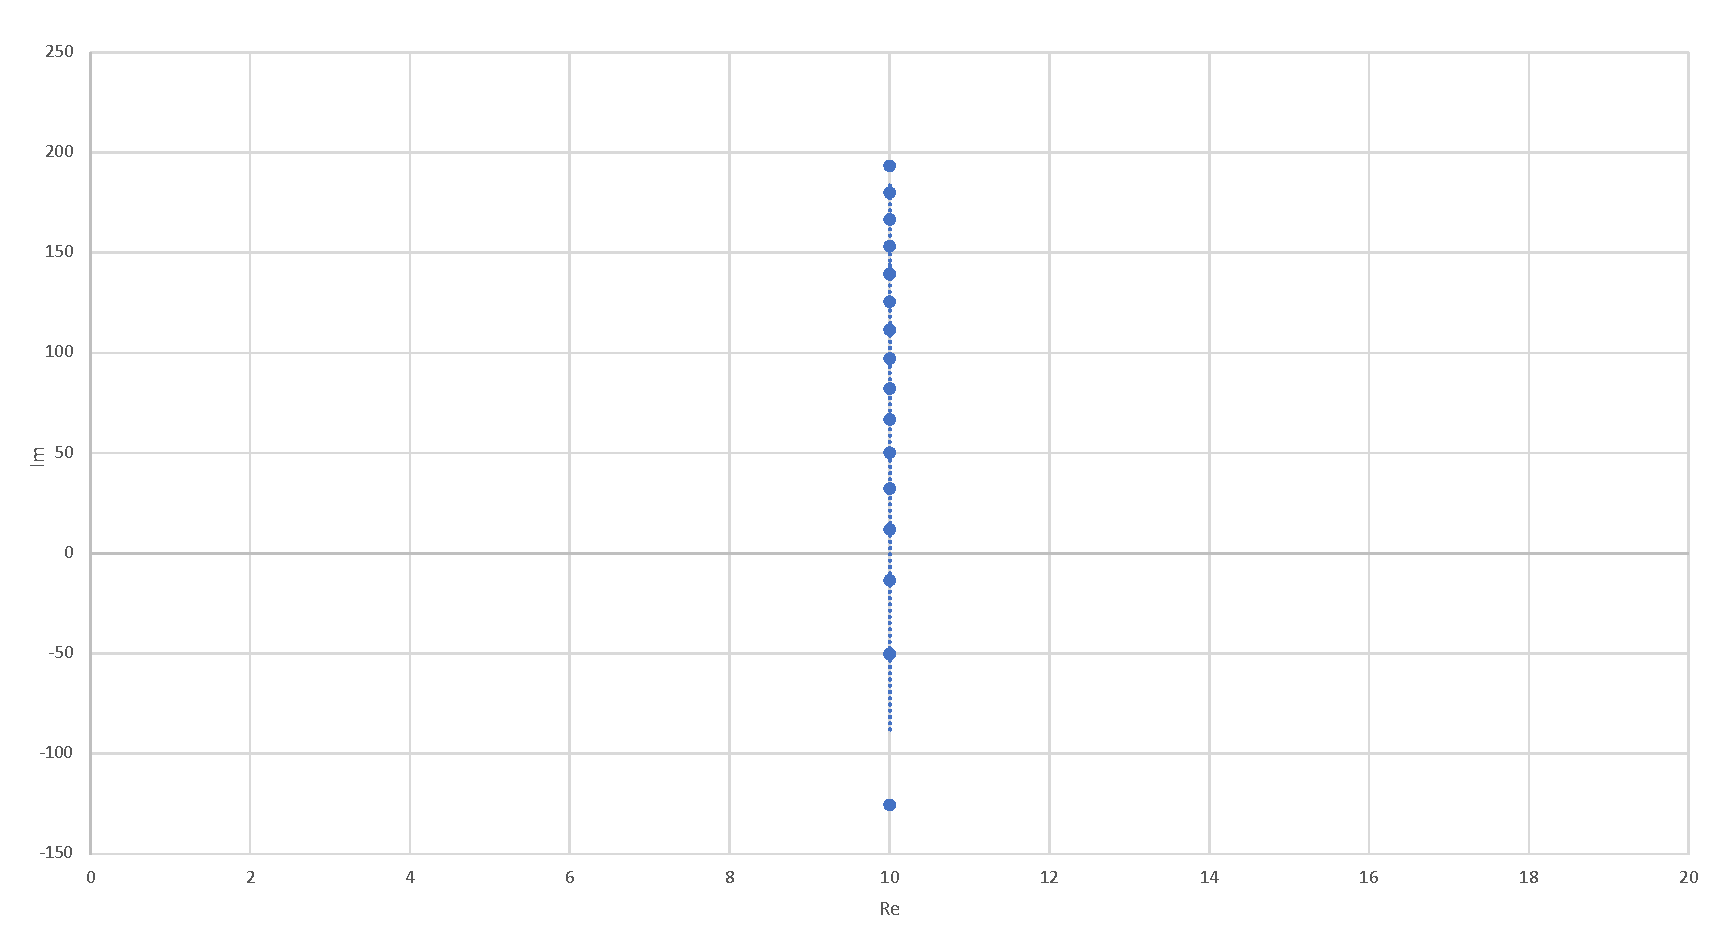
\includegraphics[scale=0.6]{./fig/fig5.pdf}
 \caption{インピーダンスの軌跡(直列)}
 \label{fig:fig7}
\end{figure}
\item \wpfig{fig5}および\wpfig{fig6}をもとにインピーダンスの軌跡を描画したものが,\wpfig{fig7}である.%5
\end{enumerate}

\newpage
\subsection{並列回路}
\begin{enumerate}
\item 測定値により導出された特性値の変化を\wptab{3}に示す.なお,インピーダンス及び偏角の値はexcelを用いて算出した.
また計算値は,小数第4位で四捨五入した.\\
$220[Hz]$付近を境にインピーダンスの増減が見られる. 

\begin{table}[hbtp]
  \centering
  \caption{インピーダンス・偏角の周波数特性(並列)}
  \label{tab:3}
  \begin{tabular}{ccc}
    \hline
    周波数$[Hz]$&インピーダンス[$\Omega$]&偏角[$rad$]\\
    \hline
    150 & 3.217 & 1.243 \\
    160 & 3.774 & 1.184 \\
    170 & 4.465 & 1.108 \\
    180 & 5.333 & 1.009 \\
    190 & 6.414 & 0.875 \\
    200 & 7.697 & 0.692 \\
    210 & 9.007 & 0.449 \\
    220 & 9.886 & 0.151 \\
    230 & 9.871 & -0.161 \\
    240 & 9.072 & -0.434 \\
    250 & 7.985 & -0.646 \\
    260 & 6.953 & -0.802 \\
    270 & 6.084 & -0.917 \\
    280 & 5.379 & -1.003 \\
    290 & 4.810 & -1.069 \\
    300 & 4.347 & -1.121 \\
    310 & 3.966 & -1.163 \\
    320 & 3.648 & -1.197 \\
    330 & 3.379 & -1.226 \\
    340 & 3.149 & -1.250 \\
    350 & 2.951 & -1.271 \\
    \hline
\end{tabular}
\end{table}
\item RLC回路の共振周波数は\wpeq{6}より$225[Hz]$であり,\wptab{3}でも$225[Hz]$近傍で抵抗の特性(偏角が0[rad]・インピーダンスが抵抗値)に近づいていることがわかる.\\
よって理論との一致が並列回路でも確認できた.
\begin{align}
\label{eq:6}
f_0&=\frac{1}{2\pi \sqrt{LC}}=\frac{1}{2\pi \sqrt{2\times 10^{-3}\cdot 250 \times 10^{-6}}} \fallingdotseq 225[Hz]
\end{align}
\item \wptab{3}の周波数変化によるインピーダンス値変化をグラフ化したものを,近似曲線と重ねて\wpfig{fig8}に示す.\\
共振周波数を軸として高周波と低周波での対照性が見られる.
\begin{figure}
 \centering
 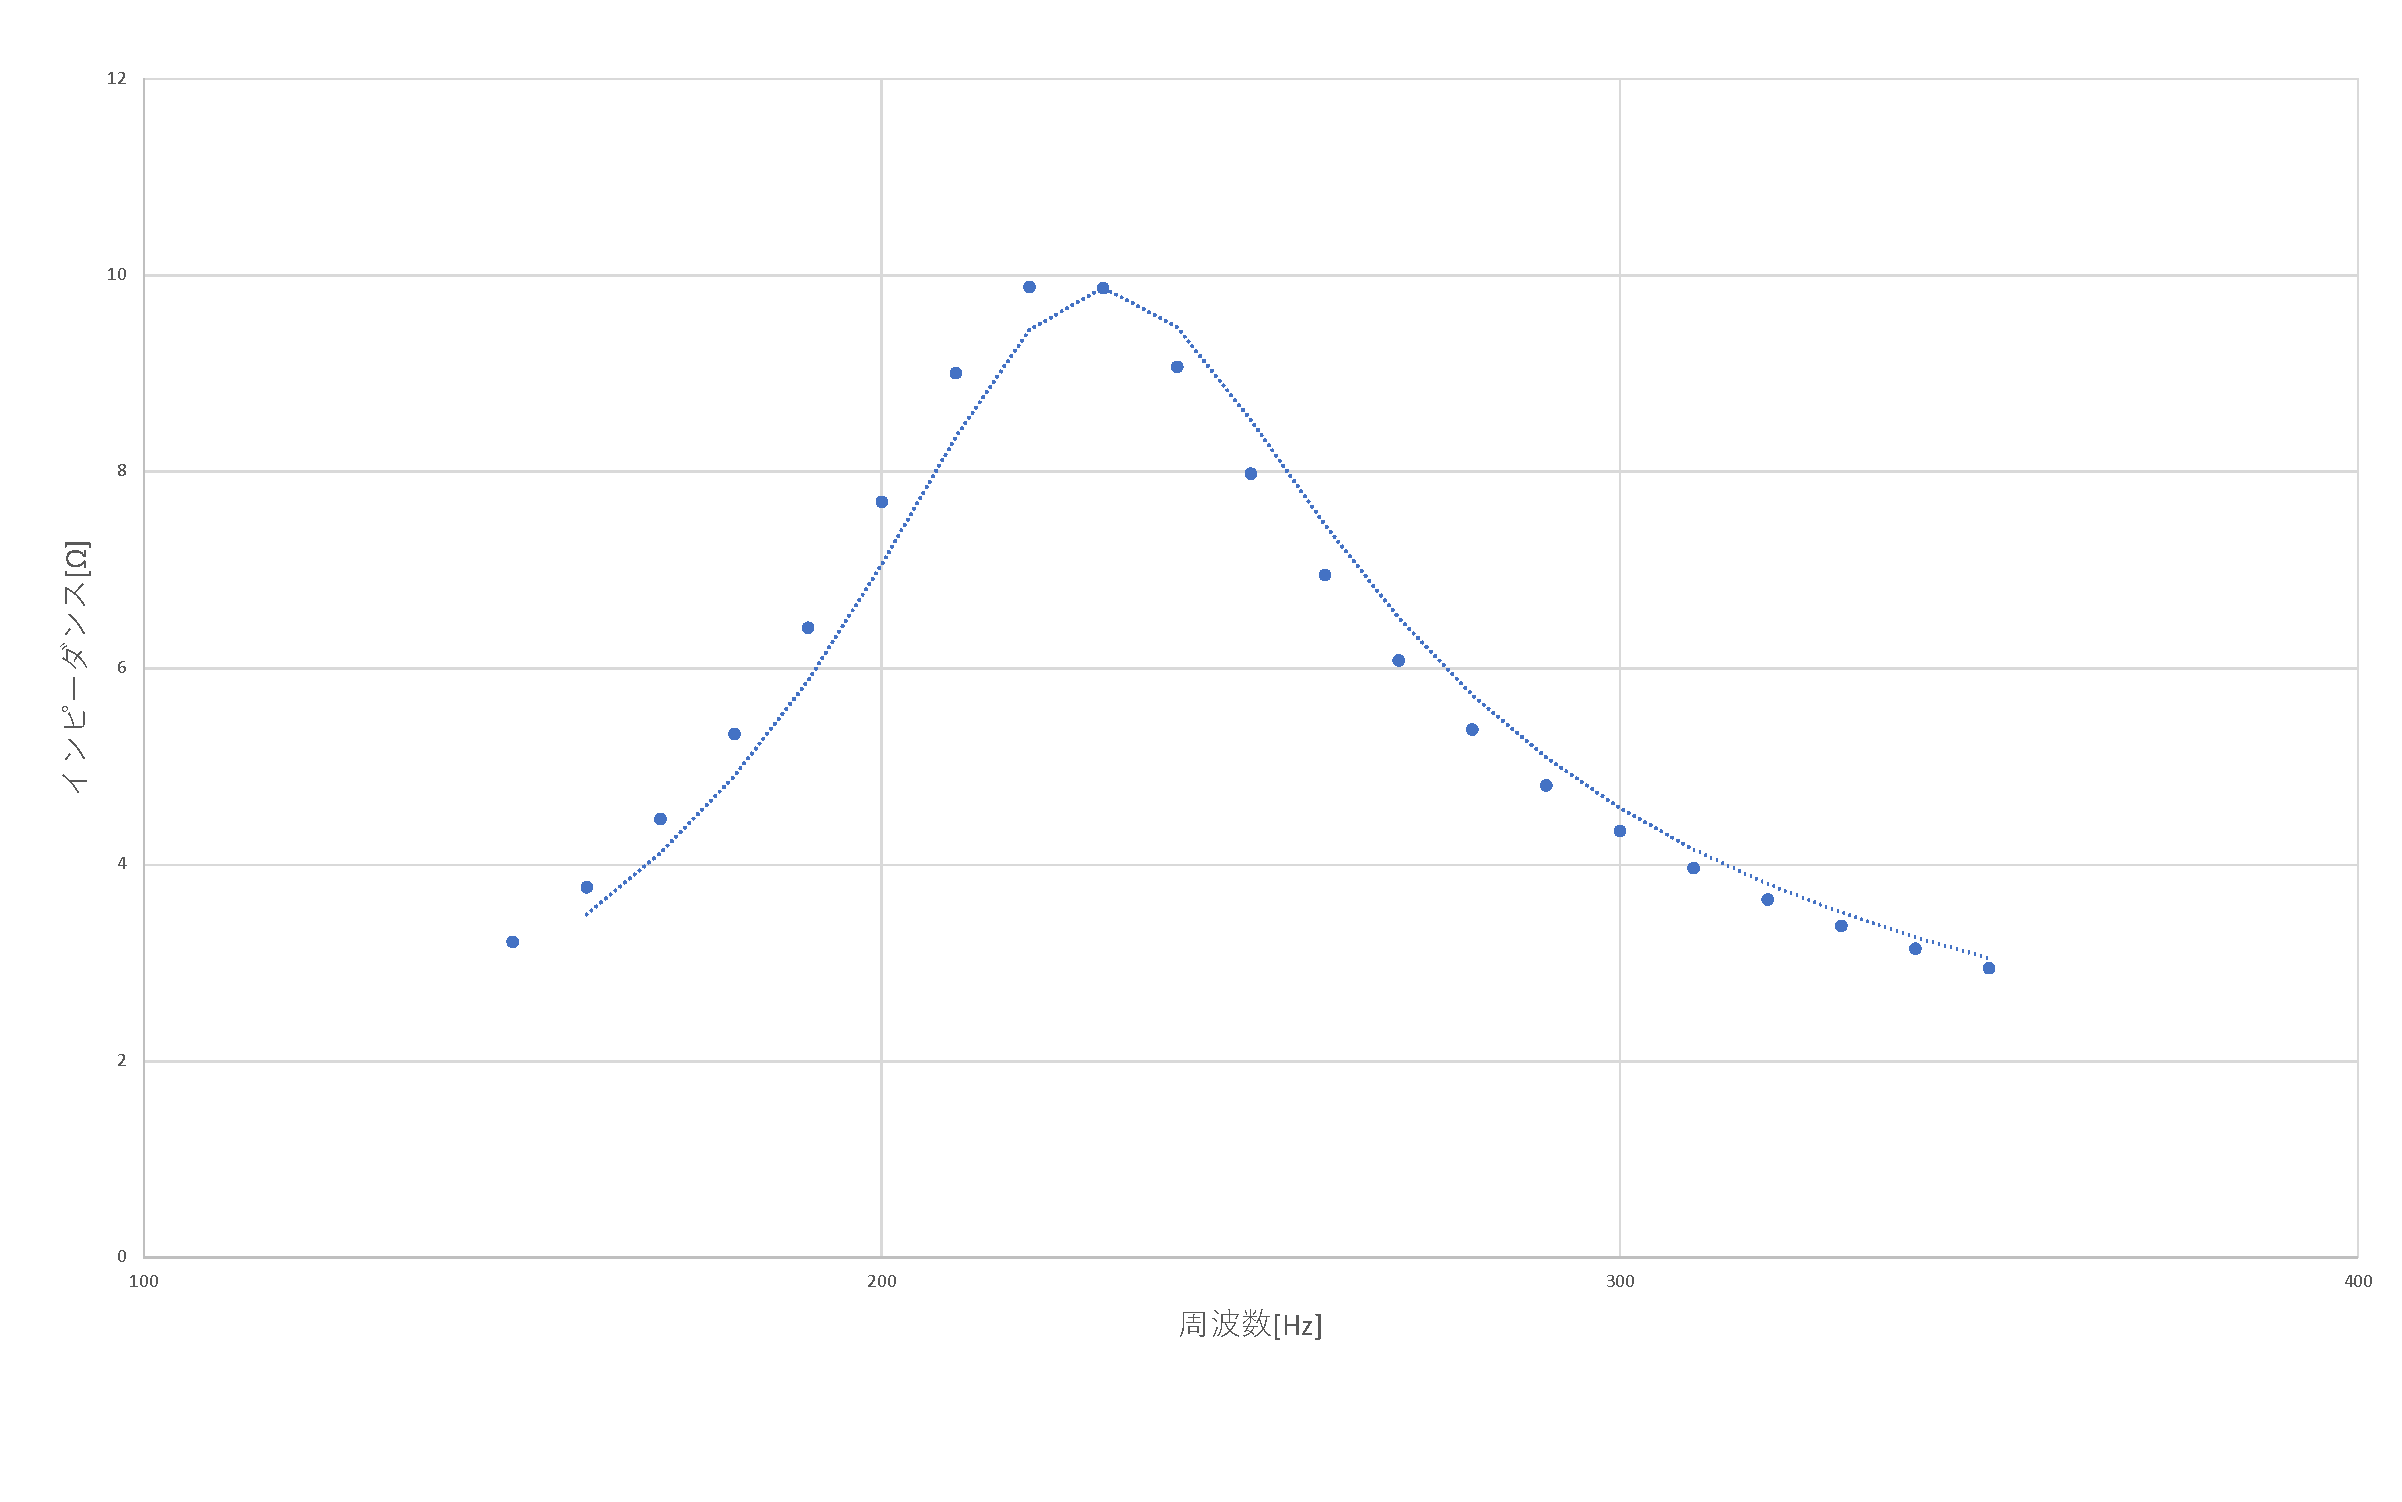
\includegraphics[scale=0.45]{./fig/graph3.pdf}
 \caption{インピーダンスの大きさの周波数特性(並列)}
 \label{fig:fig8}
\end{figure}
\item \wptab{3}の周波数変化による偏角の変化をグラフ化したものを,近似曲線と重ねて\wpfig{fig8}に示す.\\
共振周波数を境に偏角の符号がマイナスからプラスに変わっており,共振周波数付近で0の値をとっていることが読み取れる.
\begin{figure}
 \centering
 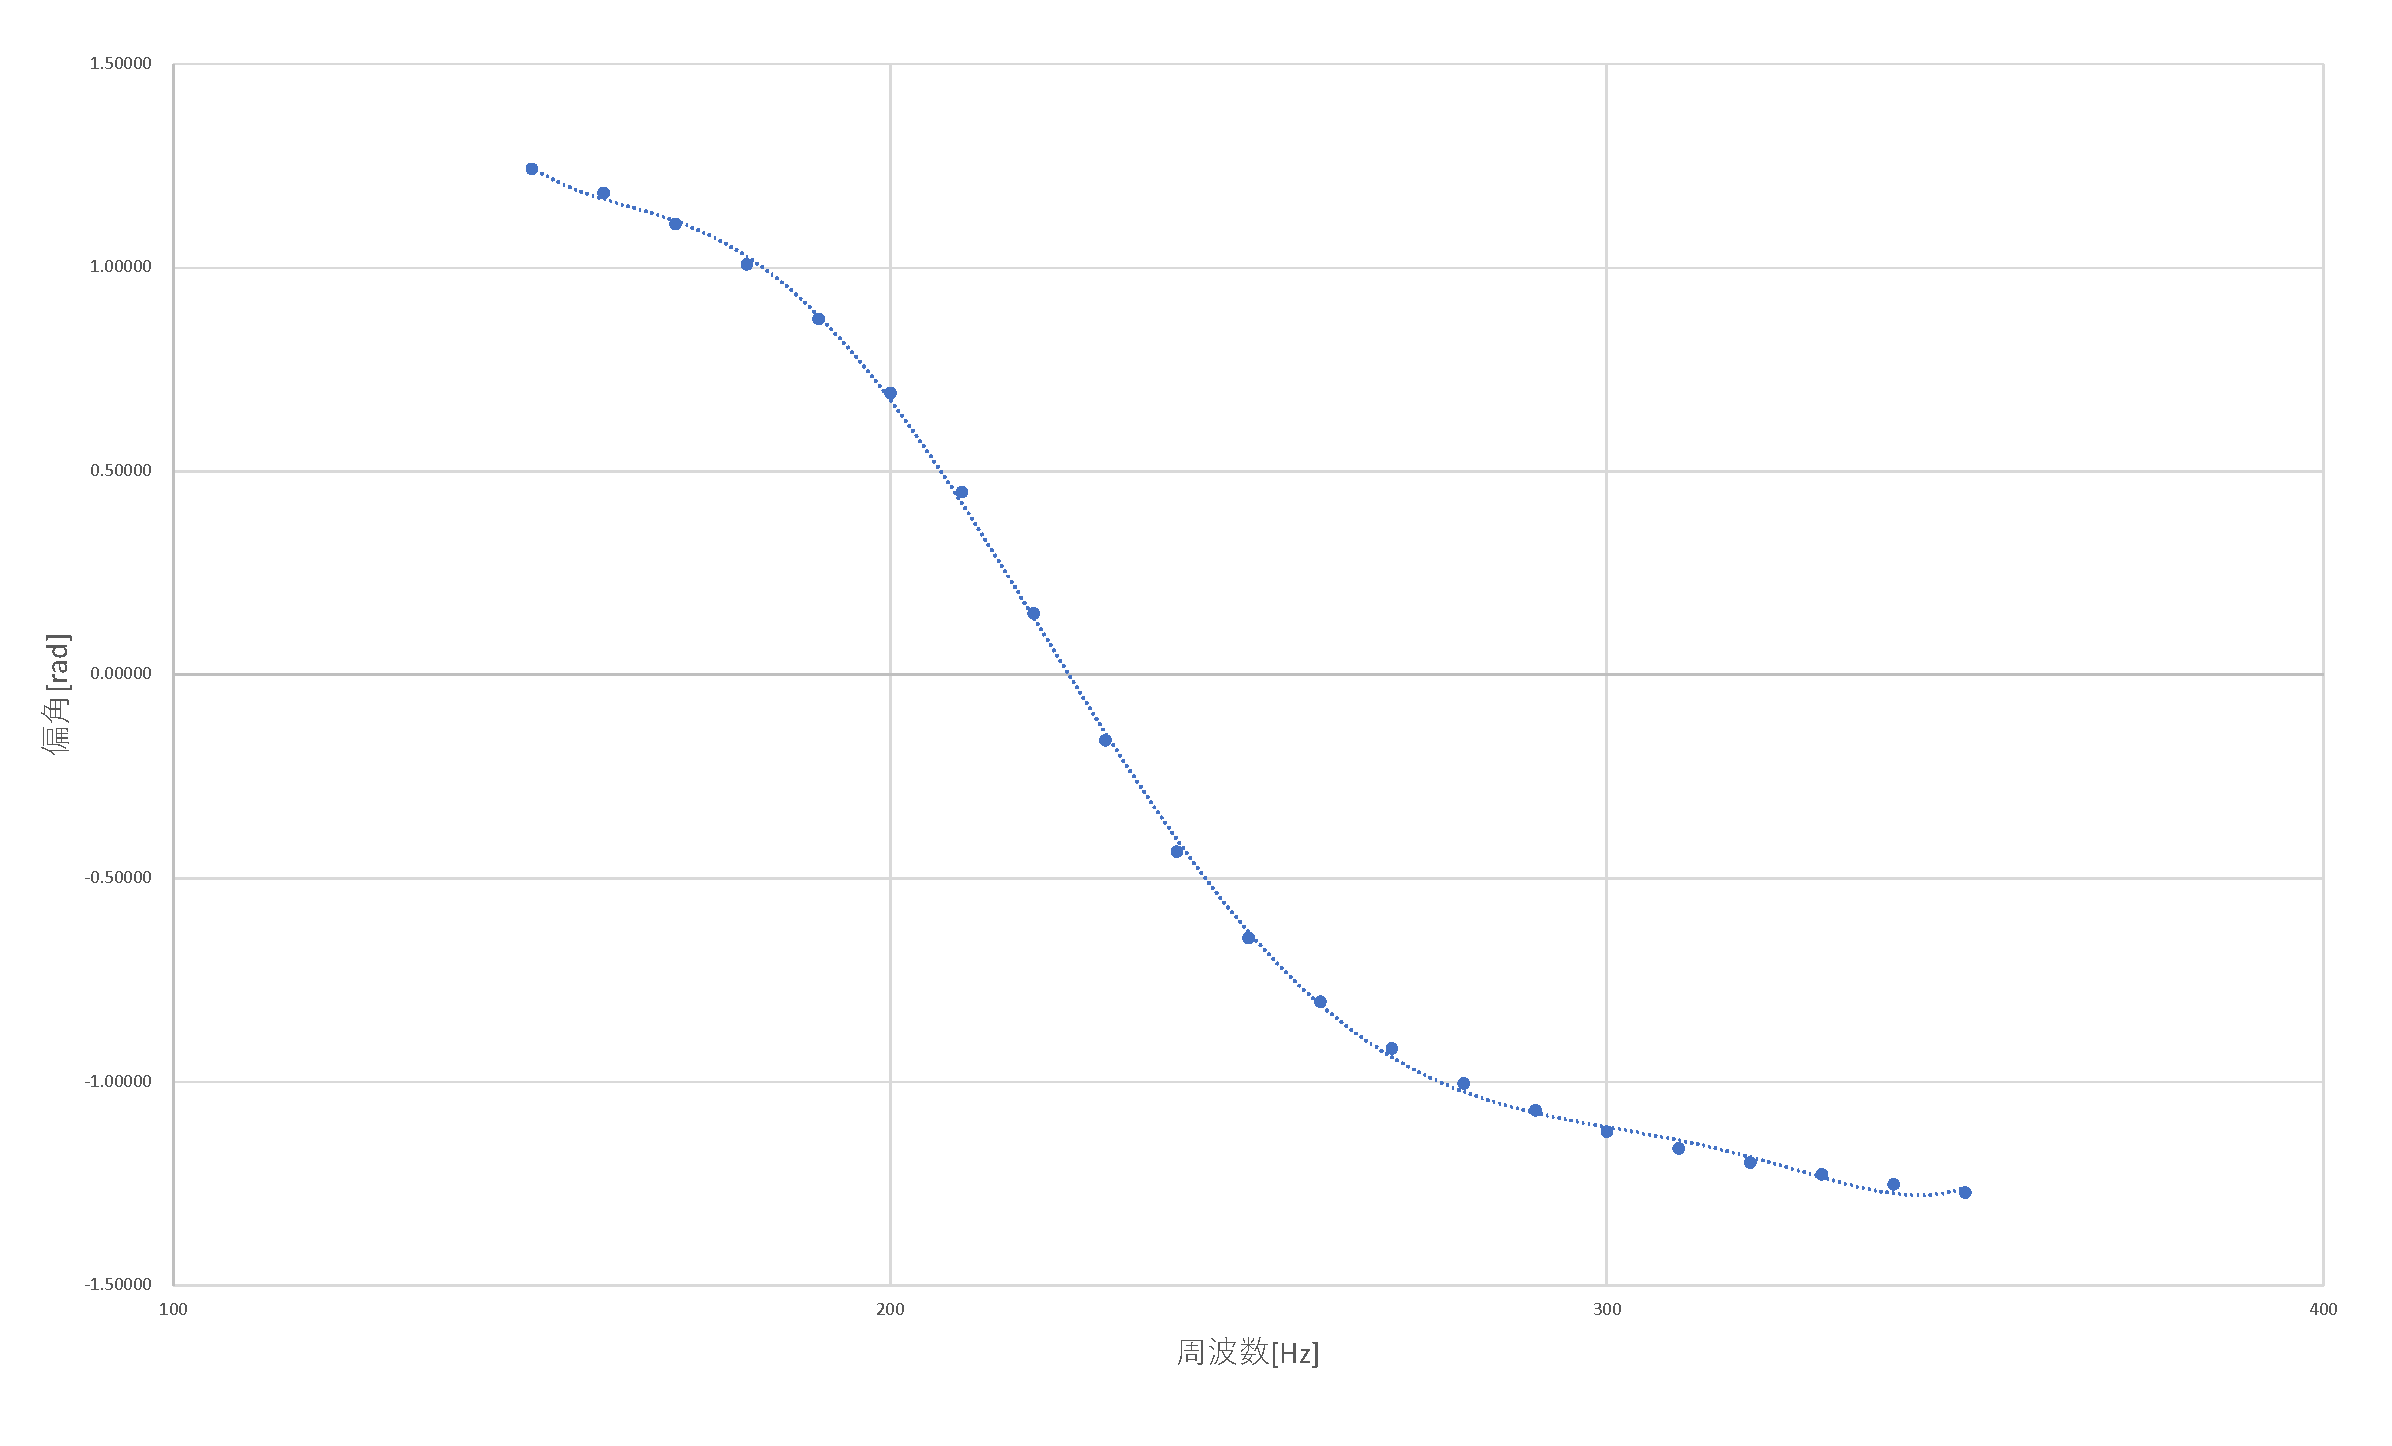
\includegraphics[scale=0.45]{./fig/graph4.pdf}
 \caption{偏角の周波数特性(並列)}
 \label{fig:fig9}
\end{figure}
\item \wpfig{fig8}および,\wpfig{fig9}よりインピーダンスの軌跡を描画すると\wpfig{fig10}のようになる.
\begin{figure}
 \centering
 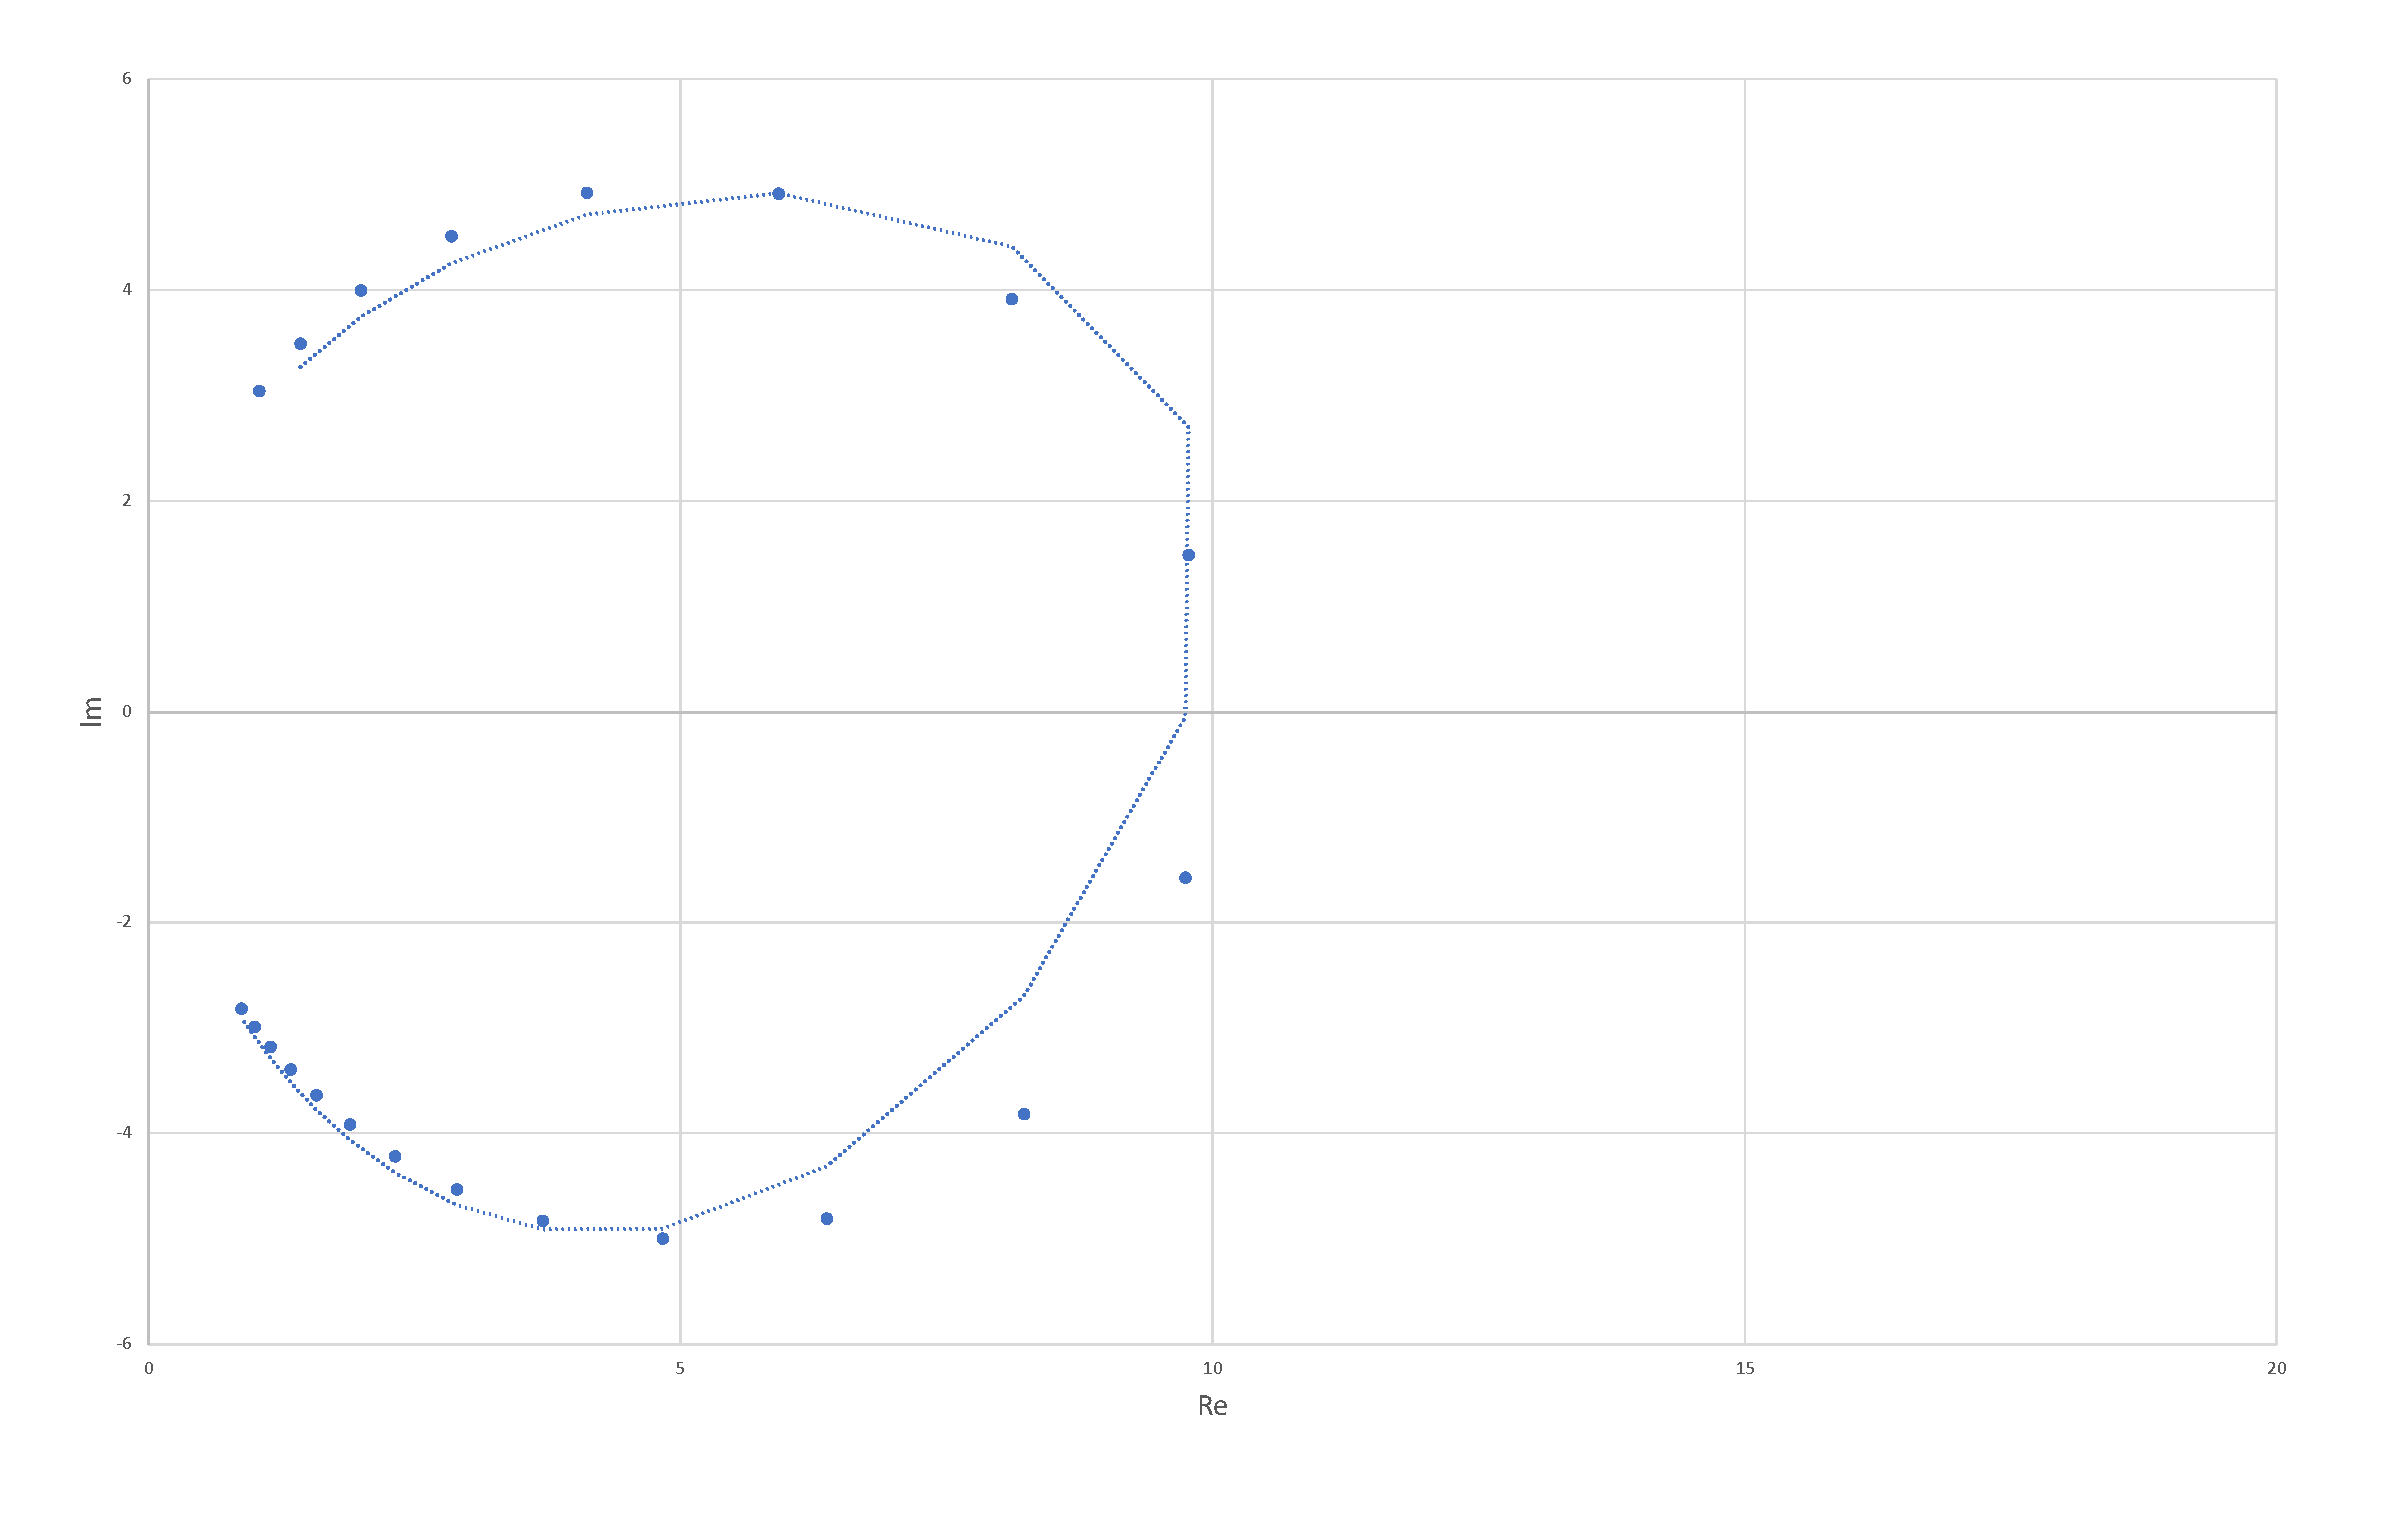
\includegraphics[scale=0.45]{./fig/fig6.pdf}
 \caption{インピーダンスの軌跡(並列)}
 \label{fig:fig10}
\end{figure}
\end{enumerate}


\section{考察}
\subsection{(直列回路)\wpeq{1},\weq{2}の導出をせよ.}
\begin{quote}
\begin{itemize}
\item 解答例:
回路全体のインピーダンスを$Z$,アドミタンスを$Y$とする,\\
\begin{align*}
\dot{I}=\dot{I}_{R}&=\dot{I}_{L}=\dot{I}_{C}\\
\dot{V}=\dot{V}_{R}&+\dot{V}_L+\dot{V}_{C}\\
\dot{V}_{R}=\dot{I}R,\quad \dot{V}_{L}&=\omega L\dot{I},\quad \dot{V}_{C}=\frac{\dot{I}}{\omega C}\\
\dot{Z}&=R+j\left(\omega L-\frac{1}{\omega C}\right)\\
&=\frac{\dot{V}_{R}}{\dot{I}}+j\left(\frac{\dot{V}_L}{\dot{I}}-\frac{\dot{V}_C}{\dot{I}}\right)\\
&=\frac{1}{\dot{I}}\left(\dot{V}_R+j\left(\dot{V}_L-\dot{V}_C\right)\right)\\
\therefore \theta_s&=\tan^{-1}\left(\frac{V_L-V_C}{V_R}\right)[rad]
\end{align*}
\item 狙い:直列回路におけるインピーダンス計算および,性質について理解を問う.
\end{itemize}
\end{quote}


\subsection{(直列回路)抵抗Rの値を大きくした際のインピーダンスの大きさ・偏角グラフの変化を考えよ.また,グラフで考察の真偽を確かめよ.}
\begin{quote}
\begin{itemize}
\item 解答例:大きさのグラフでは,最小値が抵抗の値となるため,最小値が増加する.さらに,インピーダンスの大きさは\wpeq{1}で与えられるため,Rが増加すると全体的にグラフが上に移動する.例として,インピーダンスの大きさの抵抗値特性を示したグラフを\wpfig{fig11}に示す.抵抗値の増加とともに,グラフ全体が上方に移動していることがわかる.また,共振周波数周辺での``鋭さ''(グラフの谷の狭さ)が弱まっている.\\
偏角は\wpeq{2}で与えられ,$R$の増加とともに,$V_{R}$が増加するため,$\tan^{-1}$がとる変数の値が減少していく.すなわち,偏角$\theta_{s}$も減少していくため,グラフは下に移動する.例として偏角の抵抗値特性を示したグラフを\wpfig{fig11}に示す.グラフからも先の予想通りに抵抗値増加と共に,グラフは全体的に下方に移動し,傾きが緩やかになっていることが読み取れる.
\begin{figure}
 \centering
 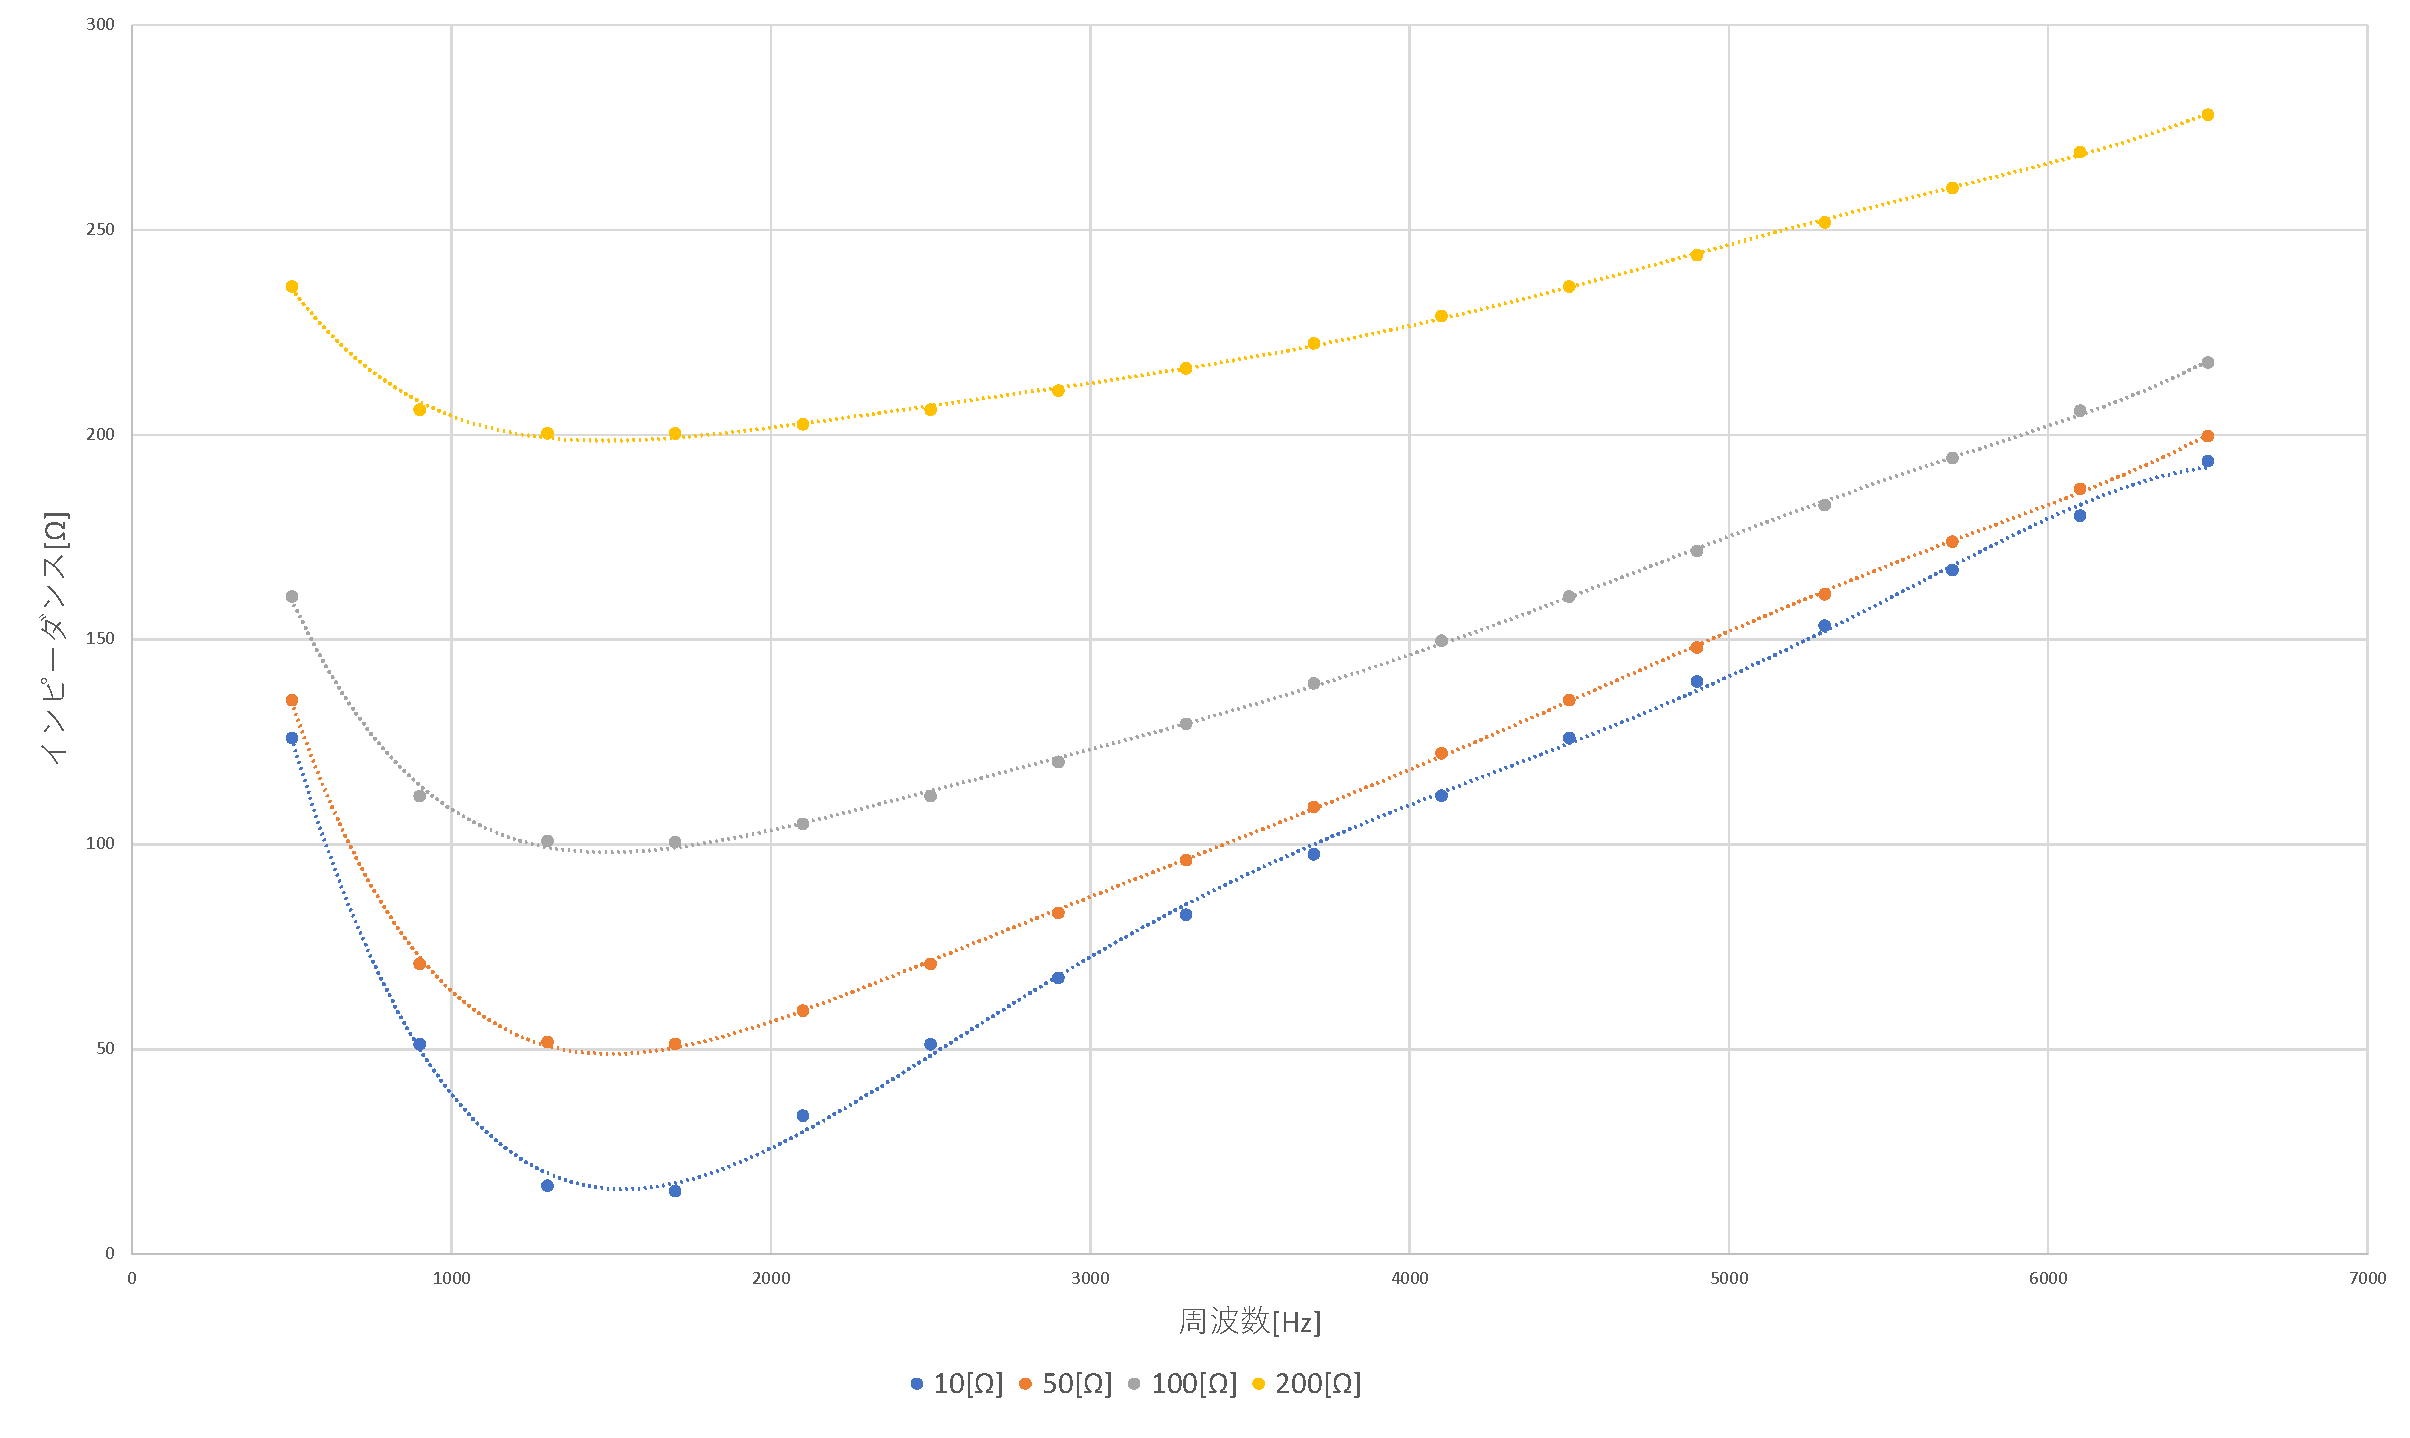
\includegraphics[scale=0.45]{./fig/graph5.pdf}
 \caption{抵抗値増加時のインピーダンスの大きさの周波数特性(直列)}
 \label{fig:fig11}
\end{figure}
\begin{figure}[hbpt]
 \centering
 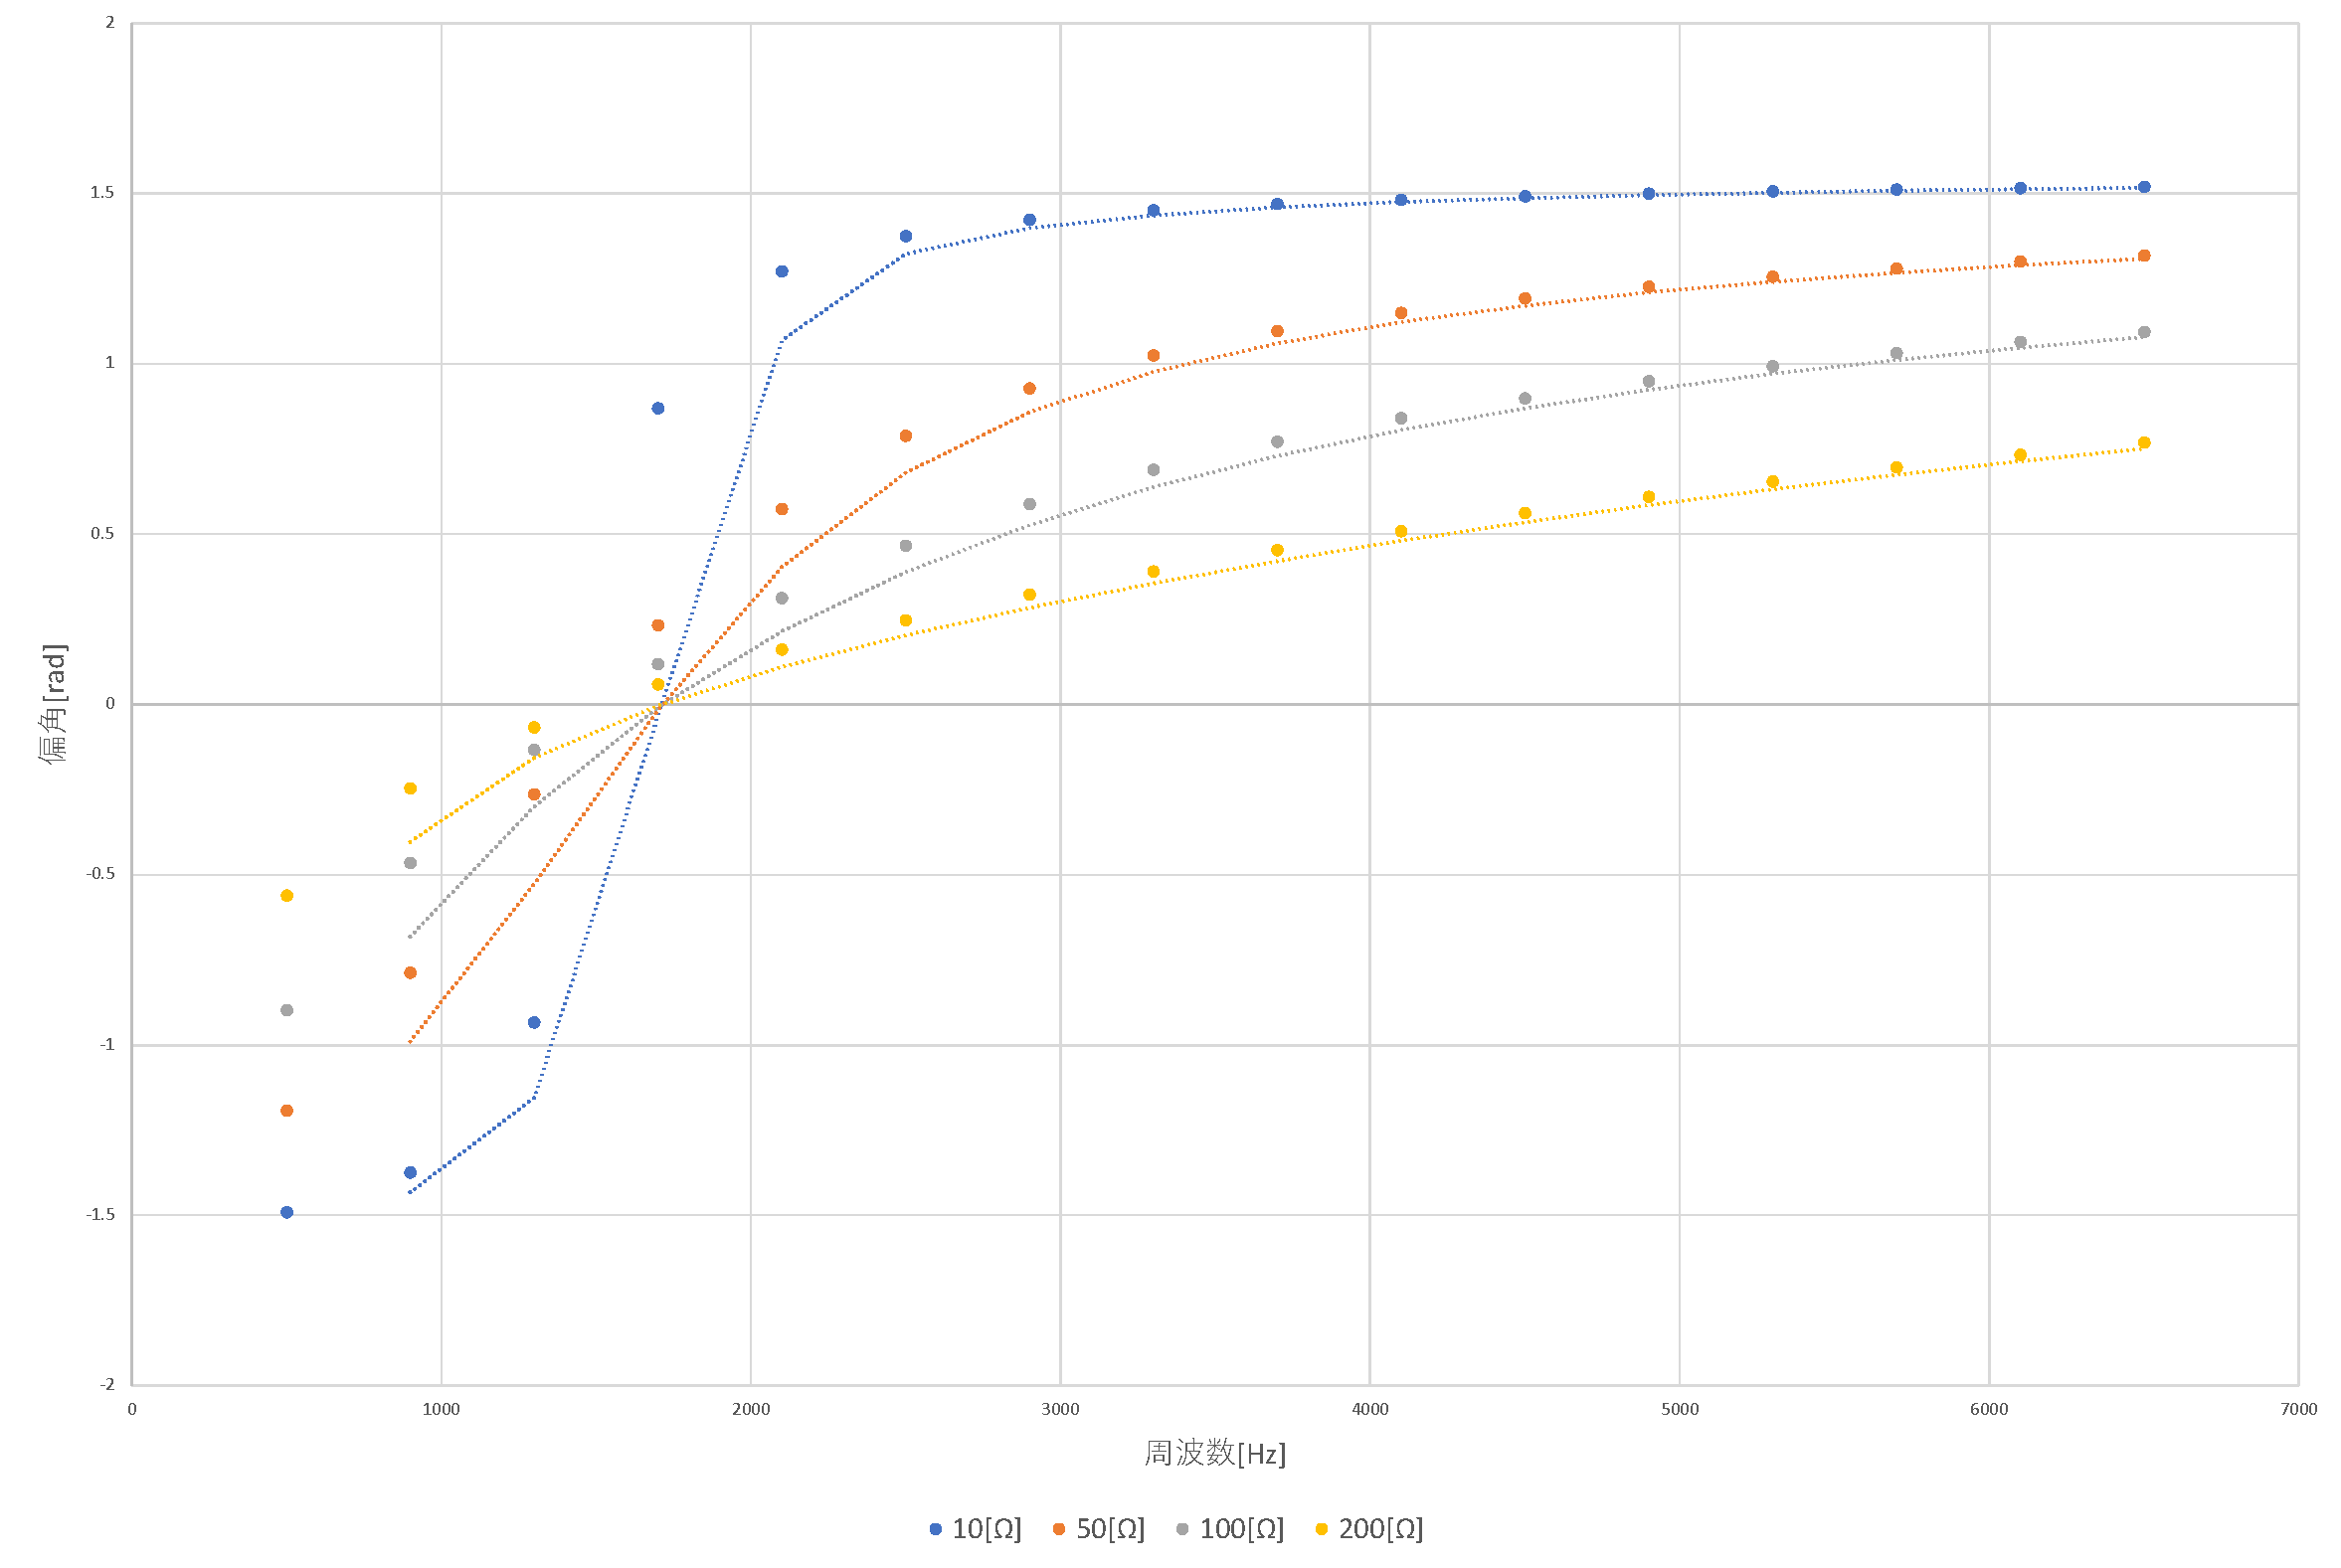
\includegraphics[scale=0.45]{./fig/graph6.pdf}
 \caption{抵抗値増加時の偏角の周波数特性(直列)}
 \label{fig:fig12}
\end{figure}
\item 狙い:抵抗値を変化させた時のインピーダンスの大きさ・偏角を導出式を用いて変化の仕方を考え,グラフを用いて変化前との違いを確認させる.
\end{itemize}
\end{quote}


\subsection{(直列回路)RLC直列共振回路では共振時に,\weq{5}が成り立つが,この$Q$の値が,回路のどのような特徴を表しているのか.さらに,グラフとの関連性についても説明せよ.}
\begin{equation}
\label{eq:7}
Q=\frac{V_{L}}{V}=\frac{V_{C}}{V}
\end{equation}
\begin{quote}
\begin{itemize}
\item 解答例:$Q$の値が大きい際,キャパシタ及びインダクタに全体の電圧に対し,多くの電圧が印加されている.つまり,グラフの共振数時の電圧が高くなるため,$Q$の値が小さい時と比べ,グラフの山の高さが高くなる.\\
また,抵抗$R$が小さければ$Q$の分母の大きさが小さくなるため,$Q$の値は大きくなる.\\
実用的に共振回路は特定の周波数の信号みを取り出して用いられることから,$Q$の値が大きいほど感度が高く,精度の良い回路だということができる.
\item 狙い:与えられた式について,自分なりに性質等を考えることができるか.
\end{itemize}
\end{quote}


\subsection{(直列回路)回路の振る舞いを低周波領域・中周波領域・高周波領域の3つに分けて考える.このとき,それぞれの領域ではどの素子の振る舞いと似ていると考えられるか.}
\begin{quote}
\begin{itemize}
\item 解答例:ここでは\wpfig{fig12}から性質を読み取る.\\
低周波では,偏角が負の値をとっているため,キャパシタの性質が強いと考えられ,\\
中周波では,一時的に偏角が$0[rad]$になることからもわかるように,抵抗の性質が強いと考えられる.\\
最後に高周波では,偏角がほぼ一定で正の値であるため,インダクタの性質が強いと考えられる.
\item 狙い:回路の反応をグラフ等から読み取り,周波数ごとに分けて近似することにより,グラフの概形を掴ませる.
\end{itemize}
\end{quote}


\subsection{(並列回路)\wpeq{3},\weq{4}の導出をせよ.}
\begin{quote}
\begin{itemize}
\item 解答例:
回路全体のインピーダンスを$Z$,アドミタンスを$Y$とする,\\
\begin{align*}
\dot{V}=\dot{V}_{R}&=\dot{V}_L=\dot{V}_{C}\\
\dot{I}=\dot{I}_{R}&+\dot{I}_{L}+\dot{I}_{C}\\
\dot{I}_{R}=\frac{\dot{V}}{R},\quad \dot{I}_{L}&=\frac{\dot{V}}{\omega L},\quad \dot{I}_{C}=\omega C\dot{V}\\
\dot{Z}&=\frac{1}{\dot{Y}}\\
&=\frac{1}{\frac{1}{R}+j\left(\omega C-\frac{1}{\omega L}\right)}\\
&=\frac{\frac{1}{R}-j\left(\omega C-\frac{1}{\omega L}\right)}{\left(\frac{1}{R}\right)^{2}+\left(\omega C-\frac{1}{\omega L}\right)^{2}}\tag{*}\\
\theta_{p}&=\tan^{-1}\left(R\left(\omega C-\frac{1}{\omega L}\right)\right)\\
&=\tan^{-1}\left(\frac{V}{I_{R}}\left(\frac{I_{C}}{V}-\frac{I_{L}}{V}\right)\right)\\
\therefore \theta_{p}&=\tan^{-1}\left(\frac{I_{C}-I_{L}}{I_{R}}\right)[rad]
\end{align*}
\item 狙い:
並列回路のインピーダンスの計算及び,性質について理解しているかを問う.
\end{itemize}
\end{quote}


\subsection{(並列回路)測定点を増加させると\wpfig{fig10}はどのような図形に近づくか.方程式を導出し,予測を確認せよ.}
\begin{quote}
\begin{itemize}
\item 解答例:測定点を増加させていくと,\wpfig{fig15}のインピーダンスの軌跡からわかるように,軌跡は円に近づいていくと考えられる.\\
方程式は,5.3の式(*)より,\\
\begin{align*}
\dot{Z}&=x+j y\\
&=\frac{\frac{1}{R}-j\left(\omega C-\frac{1}{\omega L}\right)}{\left(\frac{1}{R}\right)^{2}+\left(\omega C-\frac{1}{\omega L}\right)^{2}}\\
\therefore x&=\frac{\frac{1}{R}}{\left(\frac{1}{R}\right)^{2}+\left(\omega C-\frac{1}{\omega L}\right)^{2}},\qquad y=-\frac{\left(\omega C-\frac{1}{\omega L}\right)}{\left(\frac{1}{R}\right)^{2}+\left(\omega C-\frac{1}{\omega L}\right)^{2}}\\
x^2+y^2&=\left(\frac{\frac{1}{R}}{\left(\frac{1}{R}\right)^{2}+\left(\omega C-\frac{1}{\omega L}\right)^{2}}\right)^{2}+\left(\frac{\left(\omega C-\frac{1}{\omega L}\right)}{\left(\frac{1}{R}\right)^{2}+\left(\omega C-\frac{1}{\omega L}\right)^2}\right)^2\\
&=\frac{1}{\left(\frac{1}{R}\right)^2+\left(\omega C-\frac{1}{\omega L}\right)^{2}}\\
&=Rx\\
x^{2}+y^{2}-Rx&=0\\
\therefore \left(x-\frac{R}{2}\right)^2+y^2&=\left(\frac{R}{2}\right)^2\\
\end{align*}
上の式より,半径が$\frac{R}{2}$,中心が,$\left(\frac{R}{2},0\right)$であることがわかり,\wpfig{fig15}で示す計算による結果でもこれらを満たしていることがわかる.
\begin{figure}
 \centering
 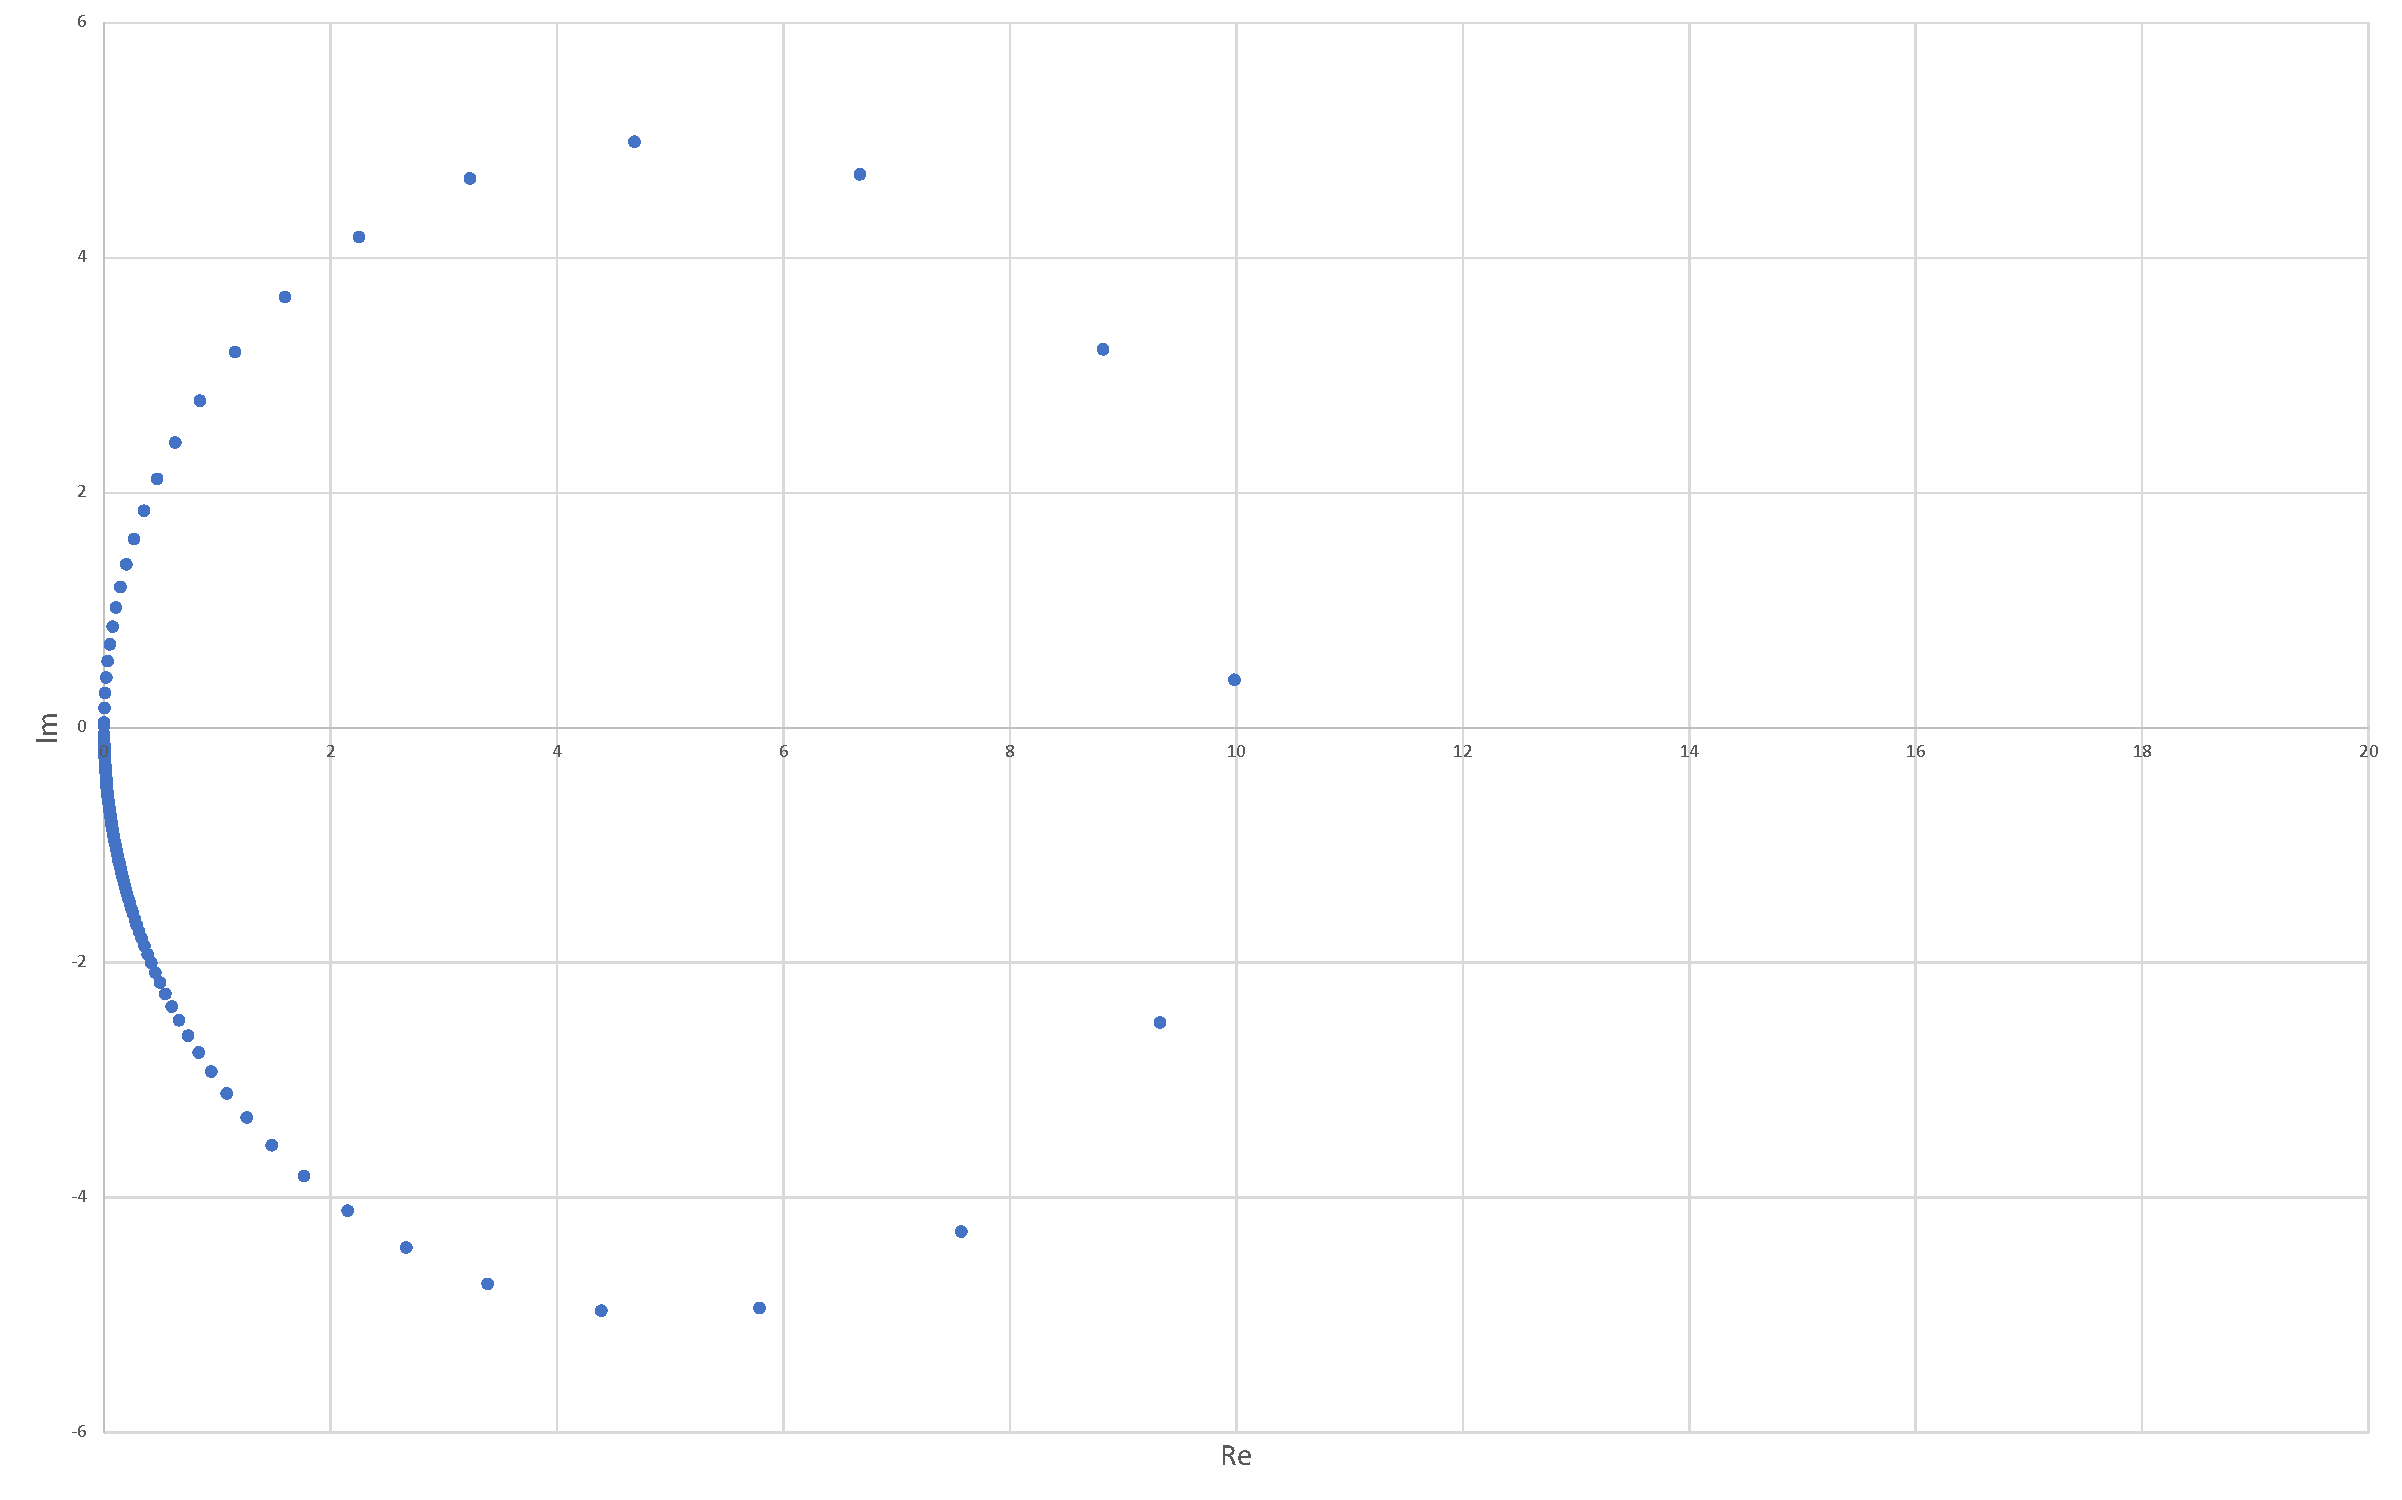
\includegraphics[scale=0.45]{./fig/fig7.pdf}
 \caption{計算点を増加させた際のインピーダンスの軌跡(並列)}
 \label{fig:fig15}
\end{figure}

\item 狙い:結果から,理論を推測させる.また,式も用いることで,定性的だけではなく,定量的にも表せるかを確認する.
\end{itemize}
\end{quote}


\subsection{(並列回路)抵抗Rの値を大きくした際のインピーダンスの大きさ・偏角グラフの変化を考えよ.また,グラフで考察の真偽を確かめよ.}
\begin{quote}
\begin{itemize}
\item 解答例:大きさのグラフでは,最小値が抵抗の値となるため,最小値が増加する.さらに,インピーダンスの大きさは\wpeq{3}で与えられるため,抵抗地が増加すると全体的にグラフが上に移動する.例として,インピーダンスの大きさの抵抗値特性を示したグラフを\wpfig{fig11}に示す.抵抗値の増加とともに,グラフ全体が上方に移動していることがわかる.また,共振周波数周辺での``鋭さ''(グラフの山の狭さ)が強まっている.これは直列回路の時とは逆の現象である.\\
偏角は\wpeq{4}で与えられ,抵抗値の増加とともに,$I_{R}$が減少するため,$\tan^{-1}$がとる変数の値が増加していく.すなわち,偏角$\theta_{s}$も増加していくため,グラフは上に移動する.例として偏角の抵抗値特性を示したグラフを\wpfig{fig11}に示す.グラフからも先の予想通りに抵抗値増加と共に,グラフは全体的に上方に移動し,傾きが急になっていることが読み取れる.これの現象もインピーダンスの大きさと同様に,直列回路と逆の動きである.また,$50[Hz]$から$200[Hz]$のグラフはあまり大きな違いが無いため,ある抵抗値を境にほぼ同じような反応をする回路を作成できるのではないか.
\begin{figure}
 \centering
 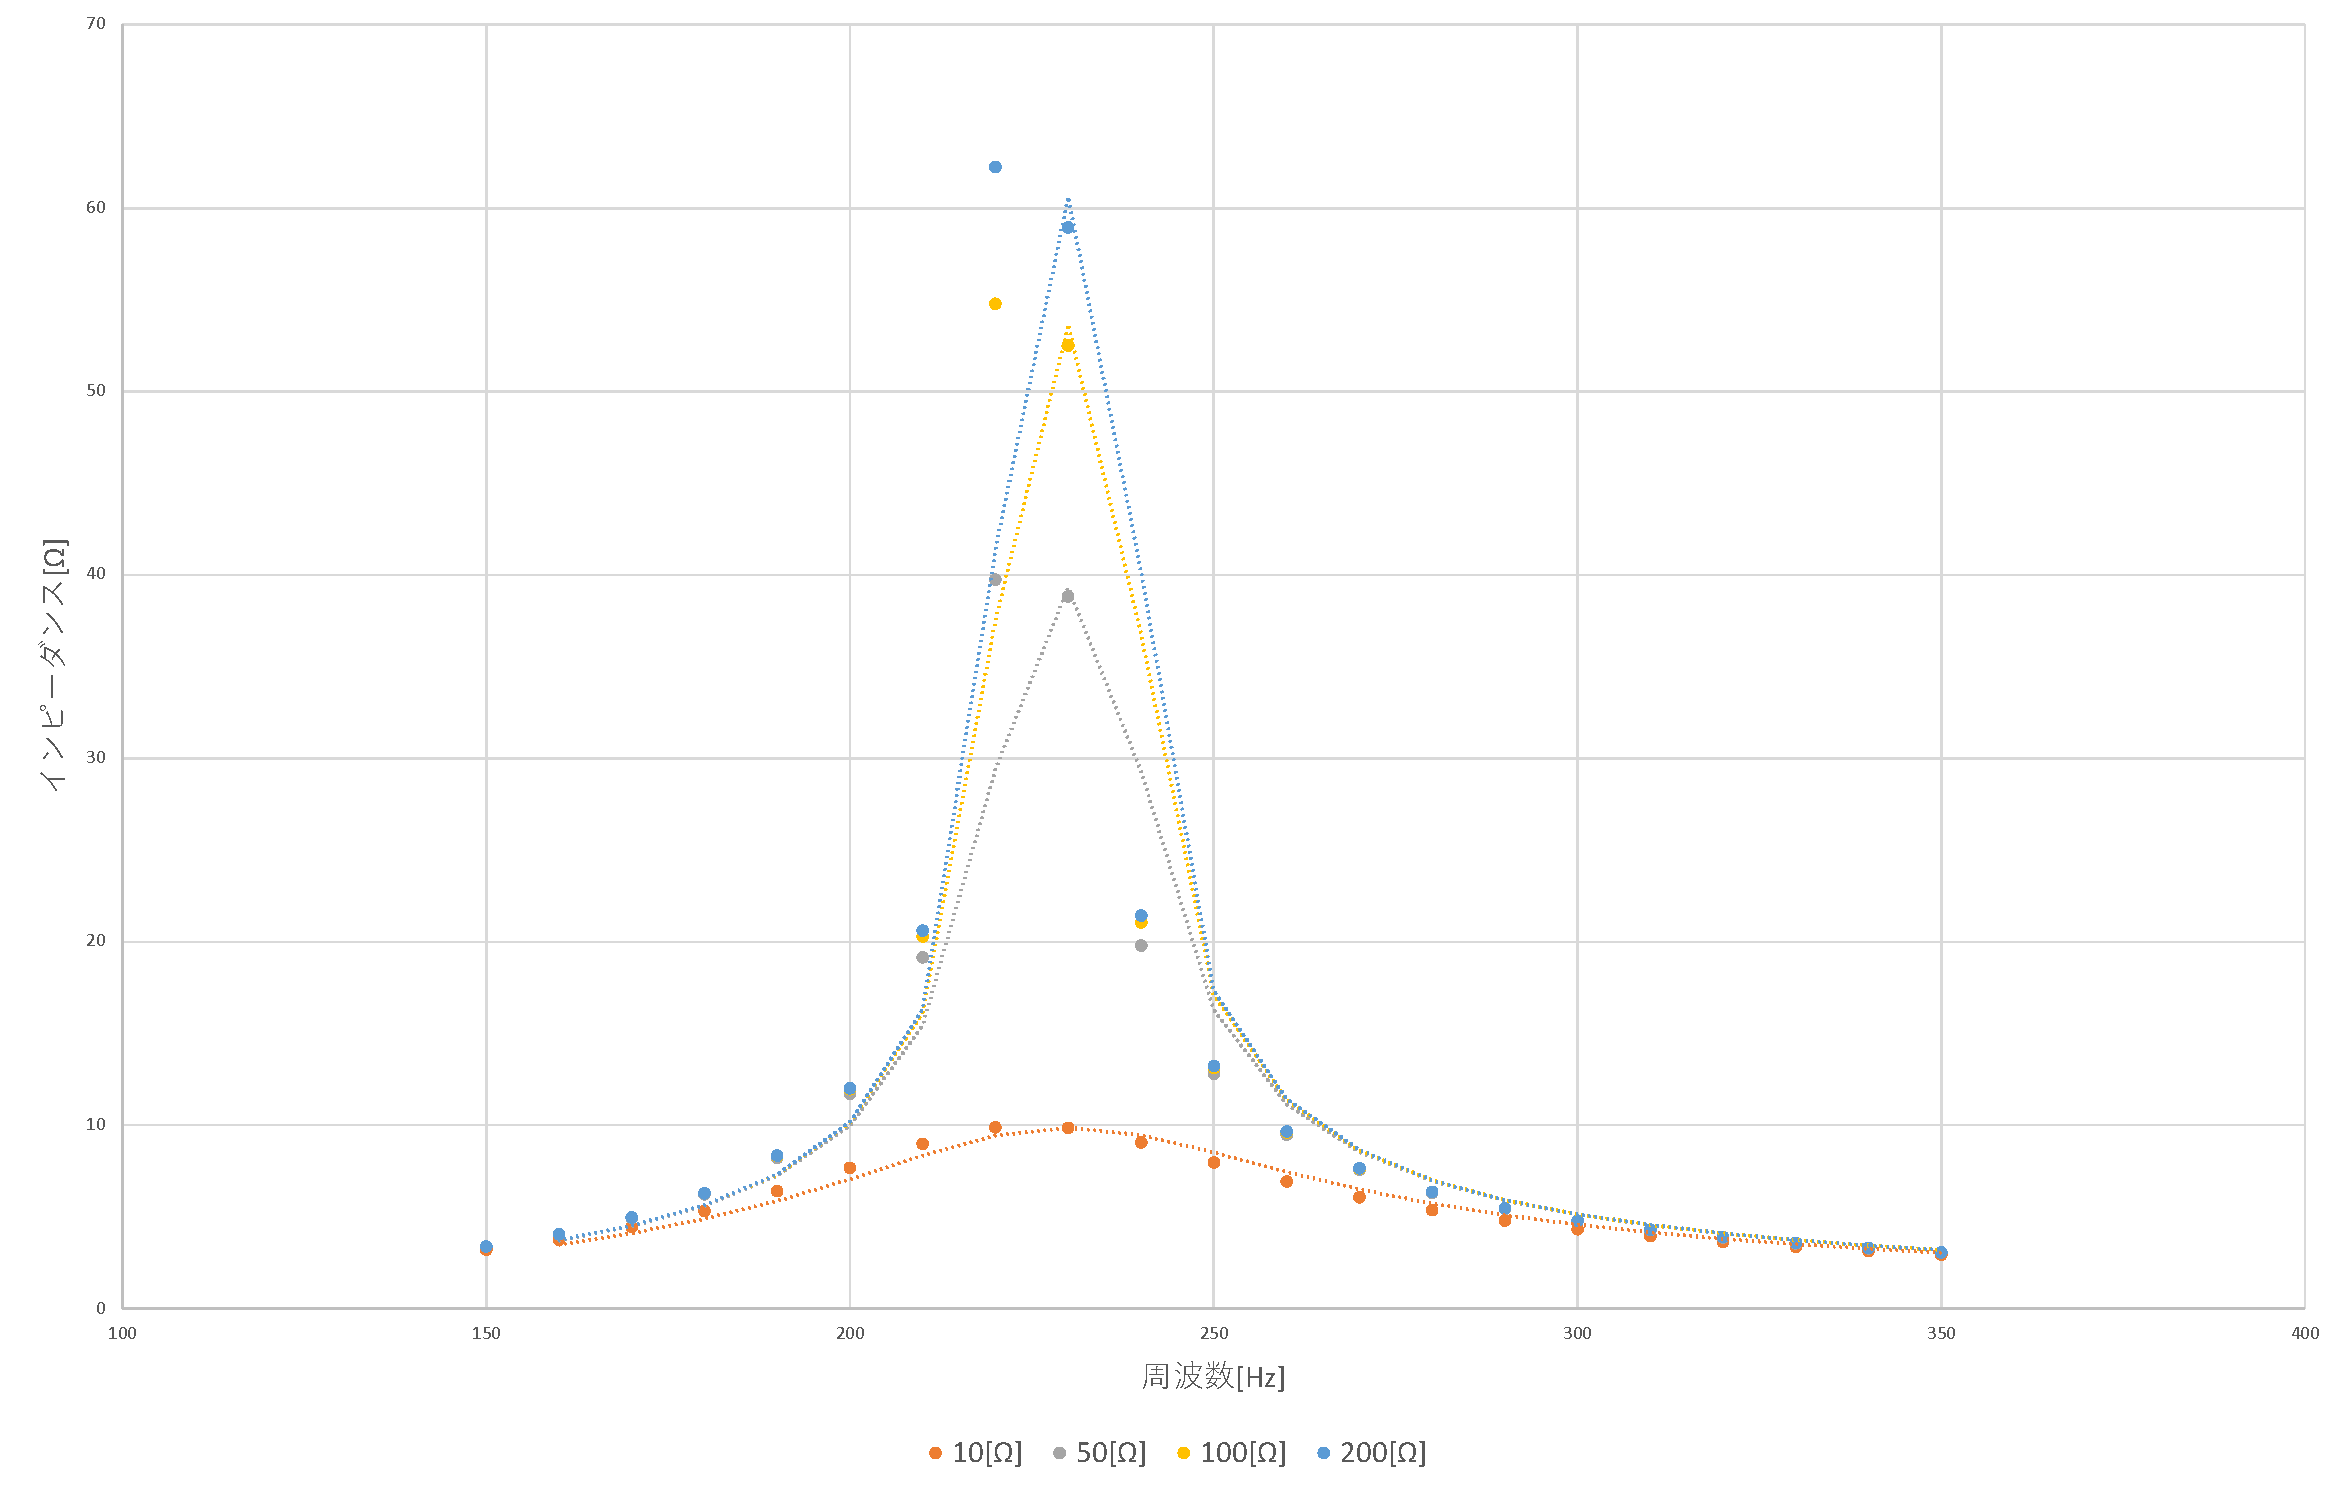
\includegraphics[scale=0.45]{./fig/graph7.pdf}
 \caption{抵抗値増加時のインピーダンスの大きさの周波数特性(並列)}
 \label{fig:fig13}
\end{figure}
\begin{figure}
 \centering
 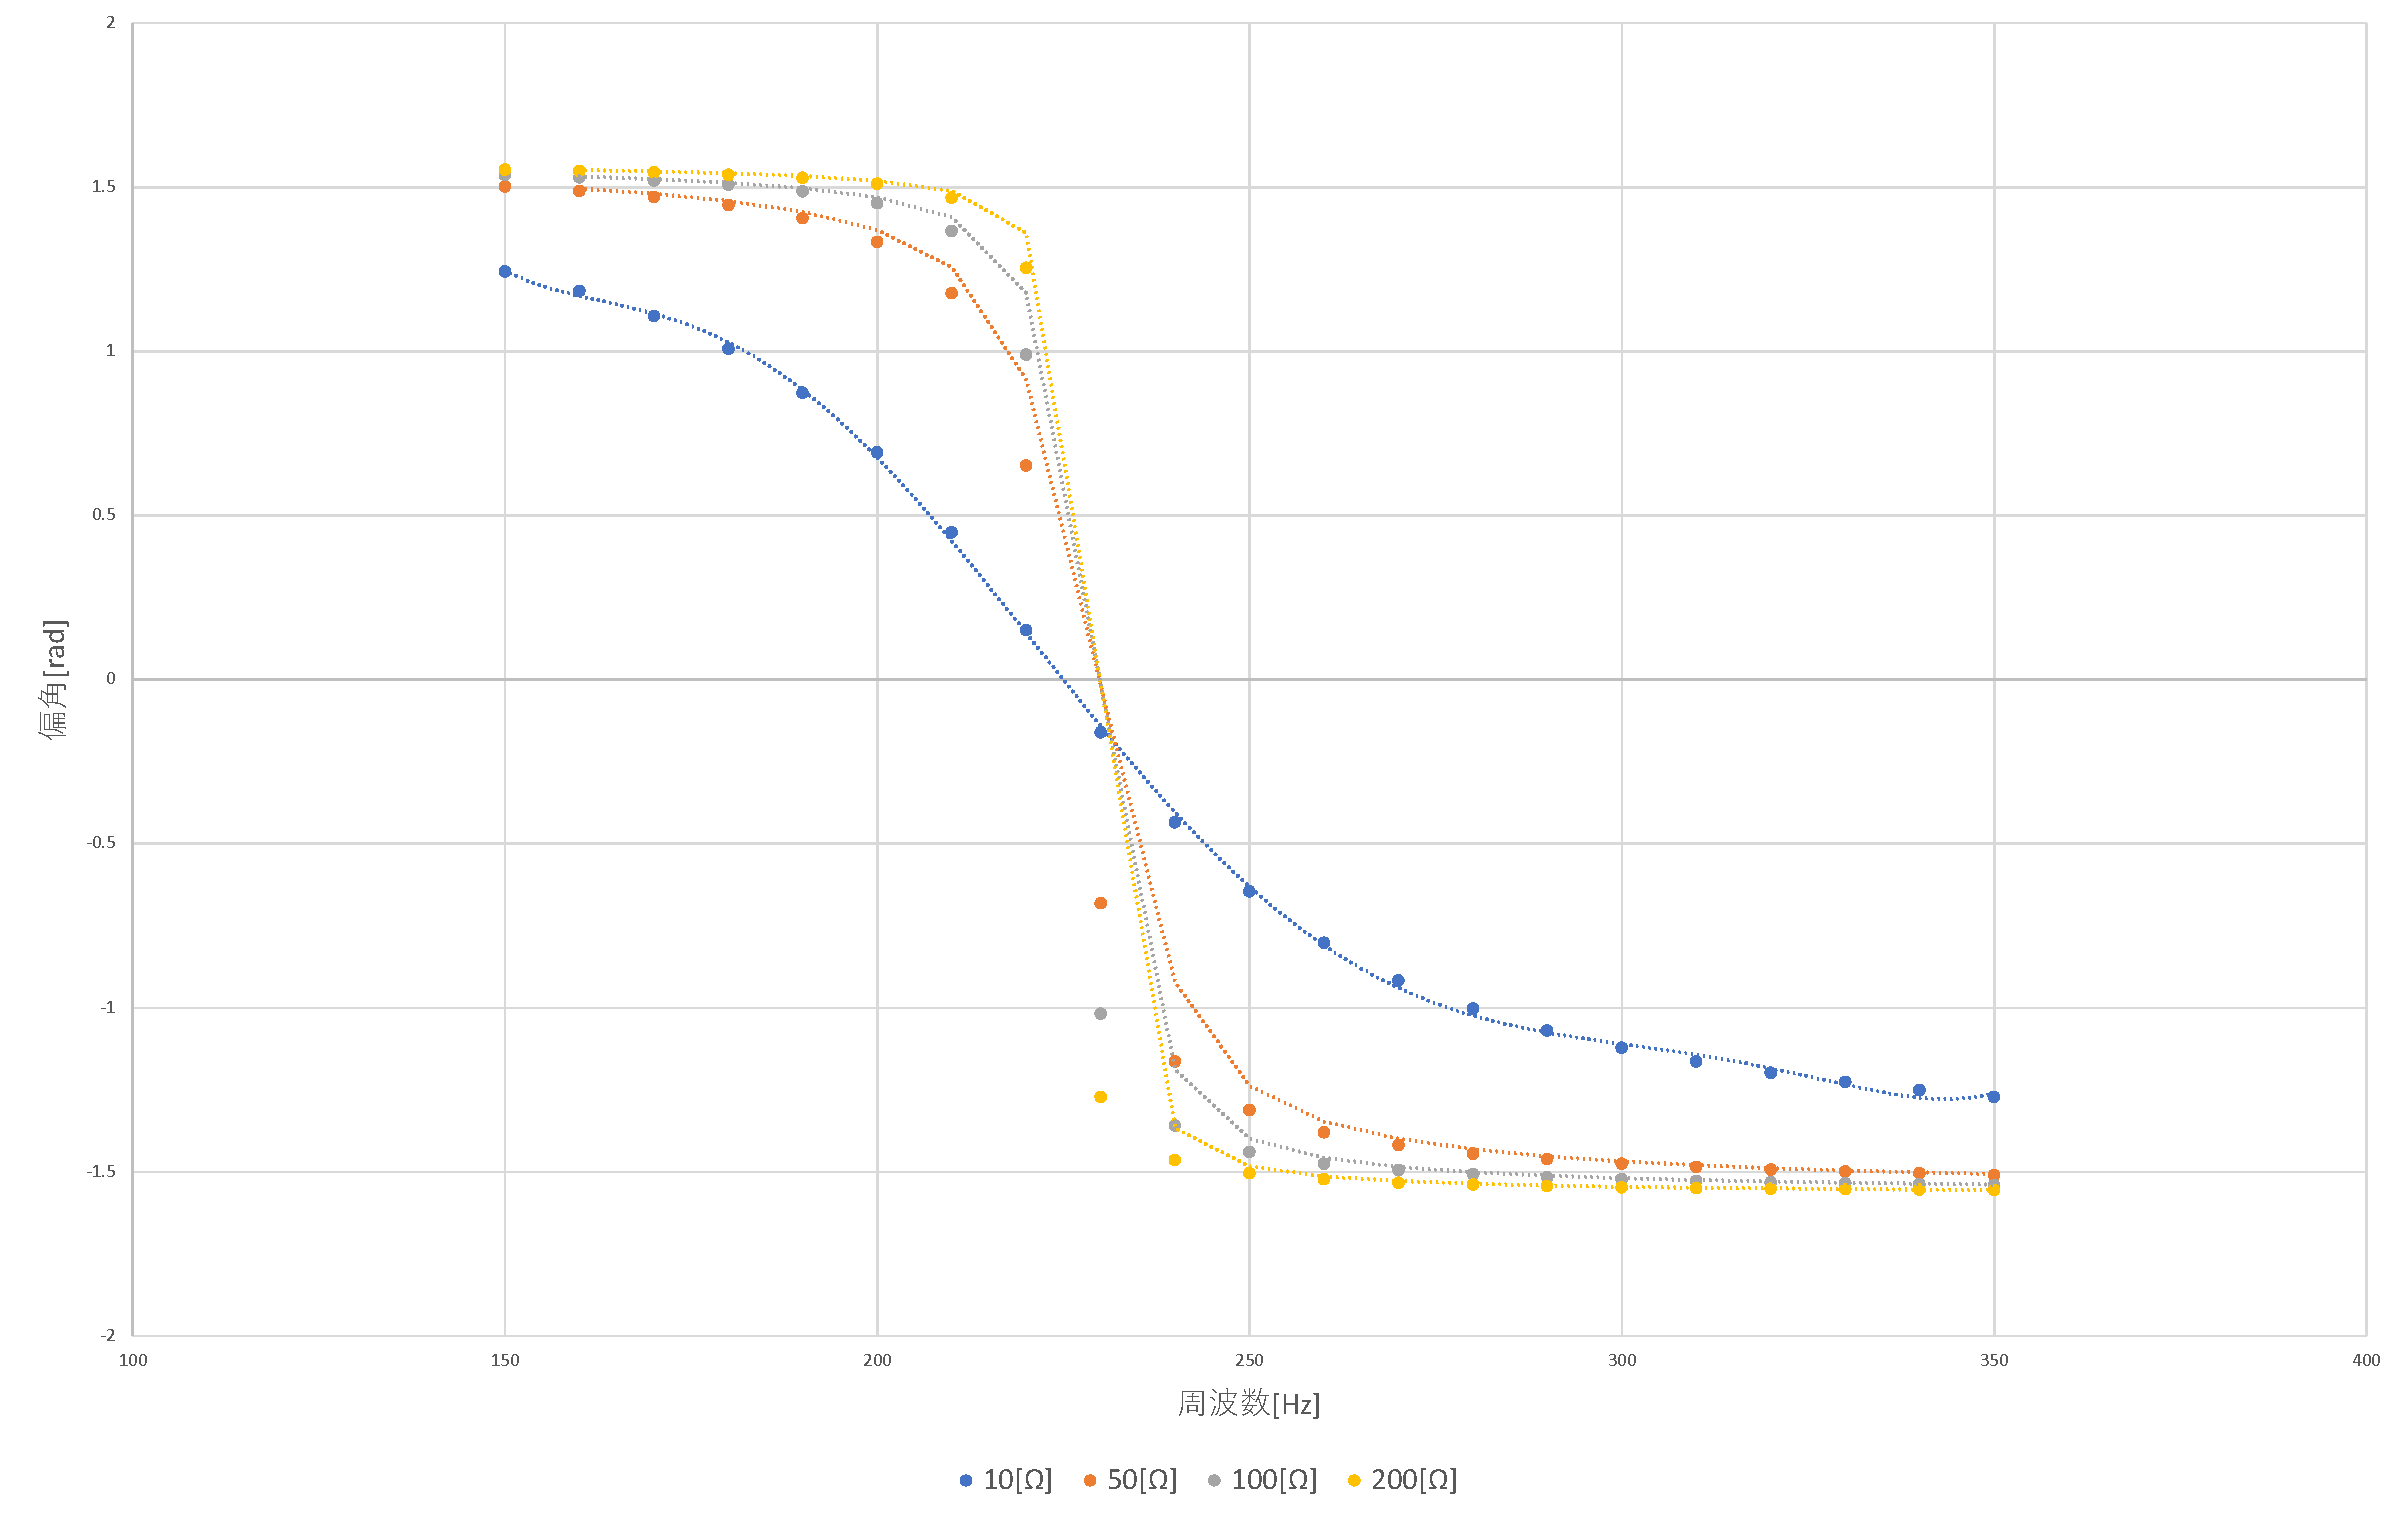
\includegraphics[scale=0.45]{./fig/graph8.pdf}
 \caption{抵抗値増加時の偏角の周波数特性(並列)}
 \label{fig:fig14}
\end{figure}
\item 狙い:抵抗値を変化させた時のインピーダンスの大きさ・偏角を導出式を用いて変化の仕方を考え,グラフを用いて変化前との違いを確認させる.また,直列回路との違いも視野に入れての考察を求める.
\end{itemize}
\end{quote}


\section{結論}
RLC回路のインピーダンスの軌跡を導出する際には,直列・並列それぞれの性質.すなわち,電流一定・電圧一定を利用することにより,測定値を用いて計算を行い,軌跡を描画することが可能である.

\end{document}
